%--------------------------------------------------------------------------
% Dokumentenklasse
%--------------------------------------------------------------------------

% disable Warning for remreset Package
% \RequirePackage{silence}
% \WarningFilter{remreset}{The remreset package}

\documentclass[
	pagesize,
	fontsize=12pt,
	paper=a4,
	oneside,
   reqno
]{scrartcl}

%--------------------------------------------------------------------------
% Standardpakete 
%--------------------------------------------------------------------------
\usepackage[ngerman]{babel}               % Deutsch Silbentrennung
\usepackage[T1]{fontenc}                  % Font Type
\usepackage[utf8]{inputenc}               % Font Encoding
\usepackage{lmodern}                      % Latin Modern Font
\usepackage{csquotes}                     % Setzen von Zitaten
\usepackage{xspace}                       % setzten von Leerzeichen nach Abkürzungen
\usepackage{microtype}                    % für glattere Seitenränder
\renewcommand*\familydefault{\sfdefault}  % Serifen lose Schrift
%\renewcommand*\familydefault{\ttdefault} % Schreibmaschinenschrift

%--------------------------------------------------------------------------
% Extra Packages

%--------------------------------------------------------------------------

% Abkürzungspaket
\usepackage{acronym}

% Symbolverzeichnis
\usepackage[symbols,nogroupskip,nonumberlist,sort=use]{glossaries-extra}

% \makenoidxglossaries

\glsxtrnewsymbol[description={Gewichtskraft}]{FG}{\ensuremath{F_{\mathrm{G}}}}
\glsxtrnewsymbol[description={Gewichtskraft in Bewegungsrichtung}]{FG1}{\ensuremath{F^{'}_{\mathrm{G}}}}
\glsxtrnewsymbol[description={Bewegungskraft des Schlittens}]{Fa}{\ensuremath{F_{\mathrm{a}}}}
\glsxtrnewsymbol[description={Pendelkraft}]{FP}{\ensuremath{F_{\mathrm{P}}}}
\glsxtrnewsymbol[description={Pendelkraft in Bewegungsrichtung}]{FP1}{\ensuremath{F^{'}_{\mathrm{P}}}}
\glsxtrnewsymbol[description={Reibkraft}]{Ff}{\ensuremath{F_{\mathrm{f}}}}
\glsxtrnewsymbol[description={Coulombsche Reibung}]{FC}{\ensuremath{F_{\mathrm{C}}}}
\glsxtrnewsymbol[description={Gesamtkraft}]{Fges}{\ensuremath{F_{\mathrm{ges}}}}
\glsxtrnewsymbol[description={Pendelmoment}]{MP}{\ensuremath{M_{\mathrm{P}}}}
\glsxtrnewsymbol[description={Gewichtsmoment}]{MG}{\ensuremath{M_{\mathrm{G}}}}
\glsxtrnewsymbol[description={Reibmoment}]{Mf}{\ensuremath{M_{\mathrm{f}}}}
\glsxtrnewsymbol[description={Gesamtmoment}]{Mges}{\ensuremath{M_{\mathrm{ges}}}}

% Mathe Pakete
\usepackage{amsmath}
\numberwithin{equation}{section}
\DeclareMathOperator{\sgn}{sgn}
\usepackage{thmtools}
\usepackage{amsfonts}
\usepackage{amssymb}
\usepackage{mathtools}
\usepackage{breqn}
\usepackage{empheq}
\usepackage{xfrac}

% Listenumgebungen
\usepackage{listings}
\usepackage{paralist}
\usepackage{enumitem}
\usepackage{adjustbox}

% Demo Text
\usepackage{blindtext}

% Farb-Pakete
\usepackage{xcolor}
\usepackage{fancyvrb}
\usepackage{colortbl}

% Farbedefinitionen
\definecolor{htw}{RGB}{120, 184, 2}
\definecolor{ccW}{RGB}{255,255,255}
\definecolor{ccR}{RGB}{197,14,31}
\definecolor{ccG}{RGB}{113,113,113}
\definecolor{ccL}{RGB}{220,220,220}
\definecolor{ccS}{RGB}{0,0,0}
\definecolor{ccB}{RGB}{68,73,159}
\definecolor{ccD}{RGB}{0,0,80}
\definecolor{grey}{RGB}{200,200,200}
\definecolor{lightGrey}{RGB}{230,230,230}

% Für erweiterte Tabellen
\usepackage{longtable}
\usepackage{tabularx}
\usepackage{float}
\usepackage{multirow}
\usepackage{makecell}
\numberwithin{table}{section}
% \setlength{\tabcolsep}{0.5em}       % for the horizontal padding
% {\renewcommand{\arraystretch}{1.8}  % for the vertical padding
% \usepackage{ragged2e}
% \newcolumntype{R}[1]{>{\RaggedRight}p{#1}}

% Einheitenpaket
\usepackage[exponent-product = \cdot]{siunitx}
\sisetup{locale=DE}
\sisetup{parse-numbers = false}

\makeatletter
\renewcommand\@dotsep{5}
\makeatother

% Pakete für Grafiken
\usepackage{graphicx}
\usepackage{wrapfig}
\usepackage{overpic}
\usepackage{epstopdf}
\usepackage{caption}
\usepackage{subcaption}
\usepackage{rotating}
\usepackage{lscape}
\numberwithin{figure}{section}
% \captionsetup[subfigure]{list=true, font=normalsize, labelformat=brace, position=top} %setup für subfigure captions

%--------------------------------------------------------------------------
% Pakete und Einstellungen für Bibliographien
%--------------------------------------------------------------------------
\usepackage[
    style=ieee,
    sorting=nty,
    sortcites=true,
    autopunct=true,
    autolang=hyphen,
    hyperref=true,
    abbreviate=false,
    backref=true,
    backend=bibtex,
    block=space,
    defernumbers=true
]{biblatex}
\bibliography{Bib/bib.bib}

%--------------------------------------------------------------------------
% Diagramm-/Grafikerstellung (TIKZ)
%--------------------------------------------------------------------------
\usepackage{pstricks}
\usepackage{tikz}
\usetikzlibrary{patterns,patterns.meta}
\usetikzlibrary{decorations.markings}
\makeatletter
\pgfkeys{/pgf/.cd,
  parallelepiped offset x/.initial=2mm,
  parallelepiped offset y/.initial=2mm
}
\pgfdeclareshape{parallelepiped}
{
  \inheritsavedanchors[from=rectangle] % this is nearly a rectangle
  \inheritanchorborder[from=rectangle]
  \inheritanchor[from=rectangle]{north}
  \inheritanchor[from=rectangle]{north west}
  \inheritanchor[from=rectangle]{north east}
  \inheritanchor[from=rectangle]{center}
  \inheritanchor[from=rectangle]{west}
  \inheritanchor[from=rectangle]{east}
  \inheritanchor[from=rectangle]{mid}
  \inheritanchor[from=rectangle]{mid west}
  \inheritanchor[from=rectangle]{mid east}
  \inheritanchor[from=rectangle]{base}
  \inheritanchor[from=rectangle]{base west}
  \inheritanchor[from=rectangle]{base east}
  \inheritanchor[from=rectangle]{south}
  \inheritanchor[from=rectangle]{south west}
  \inheritanchor[from=rectangle]{south east}
  \backgroundpath{
    % store lower right in xa/ya and upper right in xb/yb
    \southwest \pgf@xa=\pgf@x \pgf@ya=\pgf@y
    \northeast \pgf@xb=\pgf@x \pgf@yb=\pgf@y
    \pgfmathsetlength\pgfutil@tempdima{\pgfkeysvalueof{/pgf/parallelepiped offset x}}
    \pgfmathsetlength\pgfutil@tempdimb{\pgfkeysvalueof{/pgf/parallelepiped offset y}}
    \def\ppd@offset{\pgfpoint{\pgfutil@tempdima}{\pgfutil@tempdimb}}
    \pgfpathmoveto{\pgfqpoint{\pgf@xa}{\pgf@ya}}
    \pgfpathlineto{\pgfqpoint{\pgf@xb}{\pgf@ya}}
    \pgfpathlineto{\pgfqpoint{\pgf@xb}{\pgf@yb}}
    \pgfpathlineto{\pgfqpoint{\pgf@xa}{\pgf@yb}}
    \pgfpathclose
    \pgfpathmoveto{\pgfqpoint{\pgf@xb}{\pgf@ya}}
    \pgfpathlineto{\pgfpointadd{\pgfpoint{\pgf@xb}{\pgf@ya}}{\ppd@offset}}
    \pgfpathlineto{\pgfpointadd{\pgfpoint{\pgf@xb}{\pgf@yb}}{\ppd@offset}}
    \pgfpathlineto{\pgfpointadd{\pgfpoint{\pgf@xa}{\pgf@yb}}{\ppd@offset}}
    \pgfpathlineto{\pgfqpoint{\pgf@xa}{\pgf@yb}}
    \pgfpathmoveto{\pgfqpoint{\pgf@xb}{\pgf@yb}}
    \pgfpathlineto{\pgfpointadd{\pgfpoint{\pgf@xb}{\pgf@yb}}{\ppd@offset}}
  }
}
\makeatother
\usetikzlibrary{math}
\usepackage{pgfplots}
\pgfplotsset{compat=1.5}
\usetikzlibrary{intersections,positioning,arrows,automata,calc,patterns,shapes.multipart,fit,backgrounds,decorations.pathreplacing}
\usetikzlibrary{decorations,shapes.geometric}
\usetikzlibrary{matrix,calc,angles,positioning,quotes}
% \usepackage{tikz-uml}

\usepackage{pgfkeys}
\usepackage{pgfopts}
\usepackage{ifthen}
\usepackage{xstring}
\usepackage{calc}
\usepackage{pst-plot,pst-bar,pst-node} % Balkendiagramme
\usepackage{capt-of}
\usepackage{incgraph} % Fullscreen Images
\usepackage{pdfpages} % Include external pdf pages

\usepackage{latexsym}
\usepackage{censor}
\usepackage{here}
% \StopCensoring        % Auskommentiert wird der Text entschwaerzt 
% \censor{Oszilloskop}  % Befehl zum einschwärzen
\usepackage{trfsigns}   % Transformation Symbol o---o \laplace and \Laplace
\usepackage{circuitikz}

\usepackage{multido}

% Verlinkungen im Text
\usepackage{url}
\usepackage{hyperref}
\PassOptionsToPackage{hyphens}{url}
\hypersetup{hidelinks}
\urlstyle{same}

%--------------------------------------------------------------------------
% Eigene Befehle
%--------------------------------------------------------------------------
\newcommand*\widefbox[1]{\fbox{\hspace{1em}#1\hspace{1em}}} % Box für align-Umgebung

\newcommand{\mycomment}[1]{} % zum Auskommentieren von Tex-Blöcken

%------------sectioning command-------------------
% The sectioning command one level down the hierarchy from \subsubsection is called \paragraph followed by \subparagraph
% to include this in your table of contents

% Tiefe des Inhaltsverzeichnis
\setcounter{tocdepth}{3}
\setcounter{secnumdepth}{4}

% Abkürzungen durch Kommandos setzen
\newcommand{\bspw}{bspw.\xspace}
\newcommand{\bzw}{bzw.\xspace}
\newcommand{\etc}{etc.\xspace}
\newcommand{\zB}{z.\,B.\xspace}
\newcommand{\EV}{e.\,V.\xspace}
\newcommand{\zT}{z.\,T.\xspace}
\newcommand{\iVm}{i.\,V.\,m.\xspace}
\newcommand{\idR}{i.\,d.\,R.\xspace}
\newcommand{\ihv}{i.\,H.\,v.\xspace}
\newcommand{\ua}{u.\,a.\xspace}
\newcommand{\dH}{d.\,h.\xspace}
\newcommand{\vgl}{vgl.\xspace}
\newcommand{\ca}{ca.\xspace}
\newcommand{\dV}{d.\,Verf.}
\newcommand{\RNr}{Rn.\xspace}
\newcommand{\oa}{o.\,{ä}.\xspace}
\newcommand{\vC}{v.\,Chr.\xspace}
\newcommand{\nC}{n.\,Chr.\xspace}
\newcommand{\vA}{v.\,a.\xspace}
\newcommand{\eng}{engl.\xspace}
\newcommand{\tabitem}{~~\llap{\textbullet}~~}

%------------Zitate-------------------------------
\newcommand*{\zitat}[2]{%
   \normalfont\small
   \begin{quote}
   \glqq#1\grqq \par
   #2
   \end{quote}
   \normalsize
}
\newcommand*{\zitatmitueberschrift}[3]{%
   \normalfont\small
   \begin{quote} #3
   \glqq#1\grqq \par
   #2
   \end{quote}
   \normalsize
}
\newcommand*{\zitext}[2]{%
   \glqq#1\grqq\ %
   [#2]%
}

%-----------Seitendesign--------------------------
\usepackage[width=15.5cm, height=23cm, includeheadfoot]{geometry}
\geometry{paper=a4paper}
% \usepackage[left=6cm,right=1cm,top=1.5cm, bottom=1cm, includeheadfoot]{geometry}
% \newgeometry{oneside}
% \setlength{\voffset}{0cm}
\setlength{\headheight}{1.1\baselineskip} % increase headheight
\setlength{\footheight}{28.99998pt}       % increase foodheight
\setlength{\parindent}{0cm}               % Einrücken nach \newline
\setlength{\footskip}{86pt}               % Move Footer down
% \setlength{\topmargin}{0cm}
% \setlength{\marginparsep}{0.5cm}
% \setlength{\marginparwidth}{1.5cm}
% \setlength{\textwidth}{16cm}
% \setlength{\textheight}{23cm}
% \setlength{\oddsidemargin}{1cm}
% \setlength{\evensidemargin}{2cm}

%----------Kopf & Fußzeile------------------------
% \usepackage[headsepline,footsepline]{scrpage2}
\usepackage[headsepline]{scrlayer-scrpage}
\pagestyle{scrheadings}
\clearpairofpagestyles
\ihead{\headmark}
\automark{section}
\chead{}
\ohead{
\includegraphics[scale=0.09]{Bilder/HTWLogoKopfzeile.png} \nocite{Regensburg2018}}
\ifoot{Sebastian Richter\\ Aaron Zielstorff}
\cfoot{\pagemark}
\ofoot{MSS5 Computational\\ Intelligence}

%--------------------------------------------------------------------------
% Beginn des Dokuments
%--------------------------------------------------------------------------
\begin{document}

%----------Deckblatt----------------------------- 
\begin{titlepage}
   \pagestyle{empty} % setzt Pagestyle-Befehl

   % HTW Logo
   \begin{flushright}
   
\includegraphics[scale=.07]{Bilder/LogoHTWBerlin.png}  \nocite{Wikimedia2014}
   \end{flushright}

   \vspace{1cm}

   % Titel
   \begin{center}
      \Huge{\textbf{Kollisionsvermeidung eines fahrbaren Roboters\\-\\ Implementierung und Training eines neuronalen Netzes mittels Transfer-Learning}} \\
   \end{center}

   \vspace{3cm}

   % Name
   \begin{flushleft}
      \begin{tabular}{l c l }
         \textbf{Name: }&\hspace{1 cm} &\textbf{Matrikelnummer:} \\
         Sebastian Richter  & & 572906 \\
         Aaron Zielstorff   & & 567183 \\
      \end{tabular}
   \end{flushleft}

   \vspace{1cm}

   % Daten
   \begin{tabular}{l l}
      \textbf{Fachbereich:}   & FB1                                                     \\
      \textbf{Studiengang:}   & M.\xspace Elektrotechnik                                \\
      \textbf{Fachsemester:}  & 2.\xspace FS                                            \\
      \textbf{Fach:}          & MSS5 Computational Intelligence                         \\
      \textbf{Dozent:}        & Prof.\xspace Dr.\xspace -Ing.\xspace Steffen Borchers   \\
      \textbf{Abgabe am:}     & 23.\xspace September 2022                               \\ 
   \end{tabular}
\end{titlepage}
\clearpage

%--------Inhaltsverzeichnis-----------------------
\renewcommand{\contentsname}{Inhaltsverzeichnis}
\tableofcontents
\clearpage

%--------Abbildungsverzeichnis--------------------
\renewcommand{\listfigurename}{Abbildungsverzeichnis}
\renewcommand*{\figurename}{Abb.}
\listoffigures
% \clearpage

%--------Tabellenverzeichnis----------------------
\renewcommand*{\listtablename}{Tabellenverzeichnis}
\renewcommand*{\tablename}{Tab.}
\listoftables
\clearpage

%----------Symbolverzeichnis----------------------
% \printnoidxglossary[type=symbols,style=long,title={Symbolverzeichnis}]
% \clearpage

%---------Kapitel/Text----------------------------

\section{Einleitung} \label{sec:einleitung}
Diese Arbeit beschäftigt sich mit der Thematik \textit{\textbf{\glqq Künstliche Intelligenz\grqq{}}}. Künstliche Intelligenzen sind Forschungsgegenstand der Neuroinformatik. (\vgl \cite[3]{Schaeffer2021}). Speziell der Zweig der \textbf{künstlichen neuronalen Netze} (engl.\xspace Artificial Neural Network ANN) spielt immer mehr eine große Rolle für reale Anwendungsfälle. Prominente Beispiele sind unter anderem das autonome Fahren und die Worterkennung bei Sprachassistenten. (\vgl \cite[15]{Styczynski2017}). \\
Künstliche neuronale Netzwerke (im Folgenden abgekürzt mit KNN) sind Netze aus künstlichen Neuronen. Dabei handelt es sich um ein Modell nach dem biologischen Vorbild einer Nervenzelle. (\vgl \cite[136,137]{Styczynski2017}). Eine spezielle Form der neuronalen Netze sind die \textbf{Convolutional Neural Networks} (im Folgenden abgekürzt mit CNN). Der Name resultiert aus der Anwendung der Faltung  bei der Nutzung dieses Netzwerktyps. Es handelt sich auch hier um ein von biologischen Prozessen inspiriertes Konzept im Bereich des \textbf{maschinellen Lernens}. (\vgl \cite[50]{Prakash2021}). \\
In dieser Arbeit soll zunächst theoretisch das Konzept und die Funktionsweise der CNN beleuchtet werden. Dabei wird vor allem auch auf \textbf{AlexNet} als beispielhaftes CNN eingegangen, da dieses im späteren Verlauf Anwendung findet. Darauf aufbauend wird im Anschluss das \textbf{Transfer-Learning} erklärt. Auch dieses soll verwendet werden.

\begin{wrapfigure}{r}{0.5\textwidth}
    \centering
   \fbox{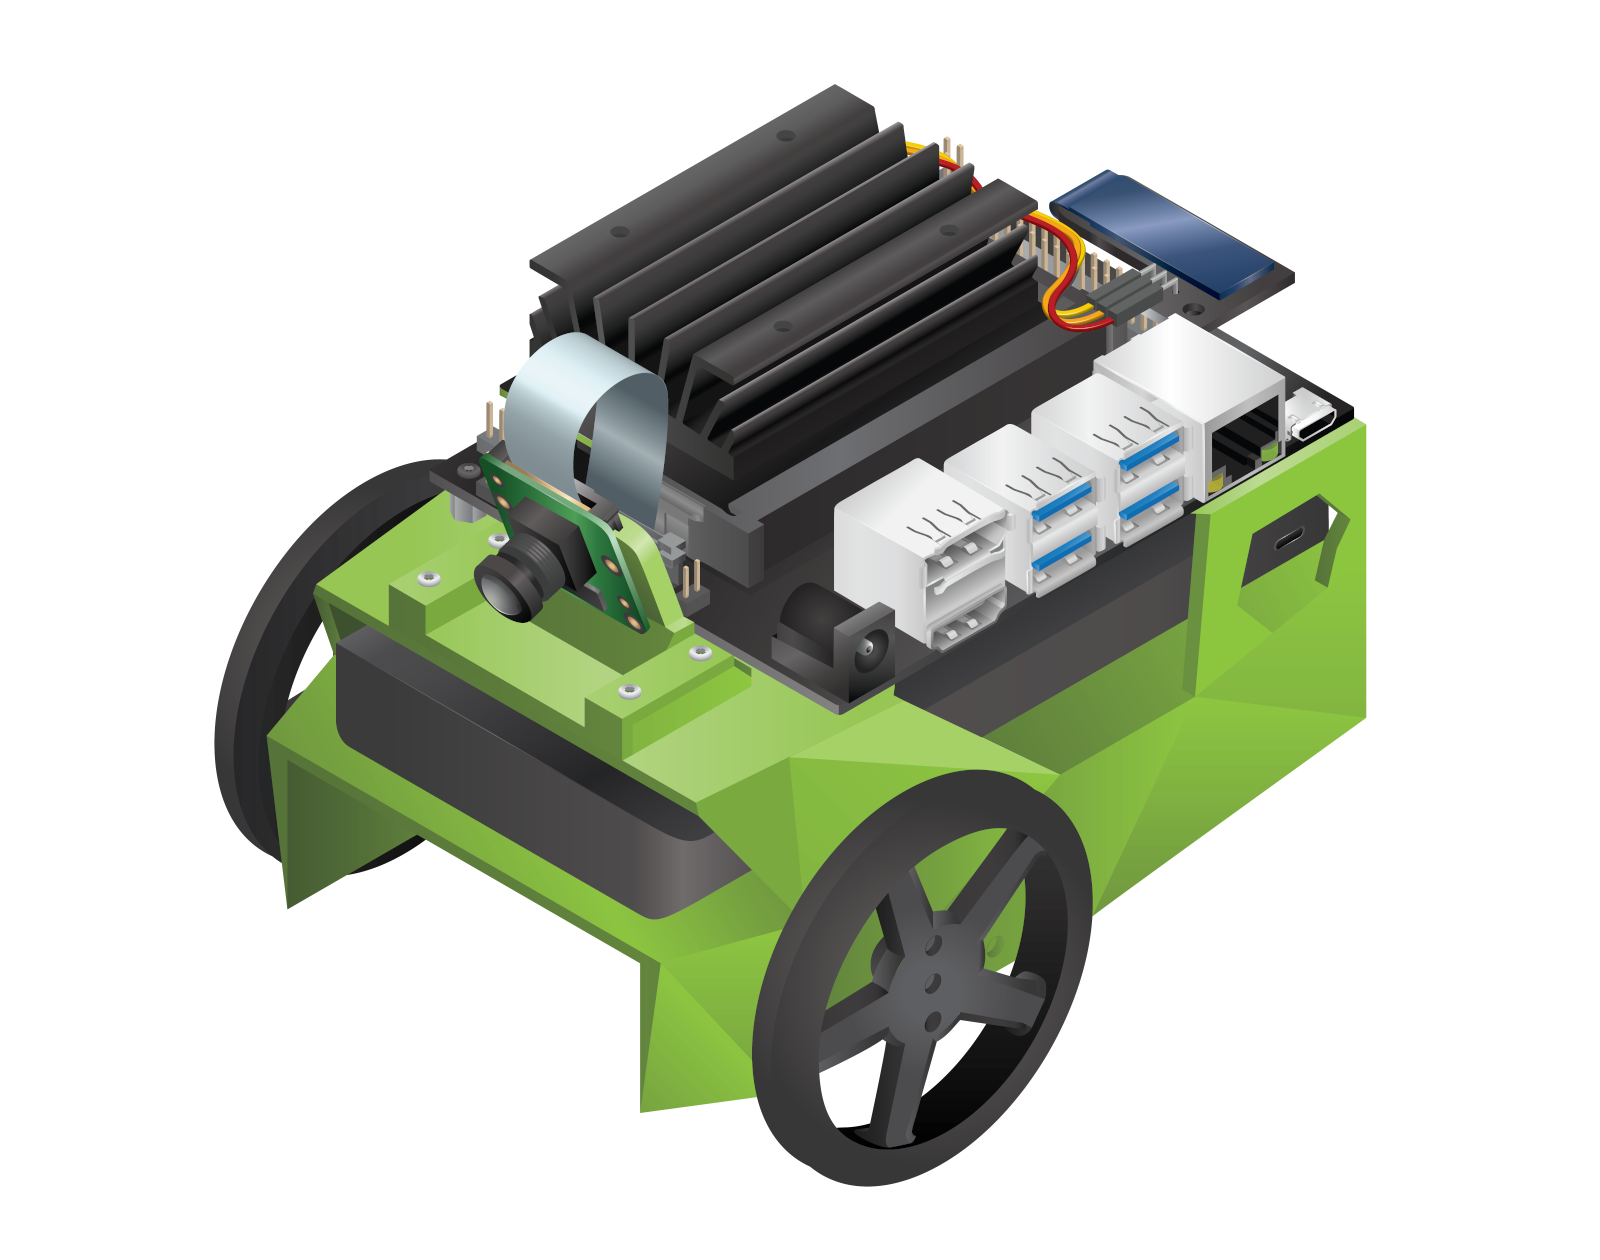
\includegraphics[width=0.48\textwidth]{Bilder/jetbot-illustration.png}}
   \caption[Illustration Jetbot Roboterfahrzeug]{Illustration des Jetbot Roboterfahrzeugs}
   \label{fig:Bild1.1}
\end{wrapfigure}

Abschließend wird die Arbeit mit der Anwendung der behandelten Konzepte an einem praktischen Versuch getestet. Hierzu sollen in Echtzeit Bilddaten von einer Kamera auf einem kleinen Roboterfahrzeug mittels CNN und Transfer-Learning ausgewertet werden, so dass das Gefährt sich kollisionfrei im Raum fortbewegen kann. Sämtliche Berechnungen als auch die Steuerung des Roboters werden auf einem \textbf{Jetson Nano} Mikrocontroller des Unternehmens Nvidia durchgeführt. Dieses ist bekannt für die Produktion von (Hochleistungs-) Grafikkarten (kurz GPU - Graphical Processing Unit). Der Jetson Controller ist ebenfalls mit einer GPU ausgestattet, die es ermöglicht rechenintensive Operationen, wie \zB die Berechnung von neuronalen Netzen durchzuführen. \\
Die \autoref{fig:Bild1.1} zeigt den Jetson Nano Controller auf dem Roboterfahrzeug \textit{\glqq Jetbot\grqq{}} inklusive einer kleinen Weitwinkelkamera.

\section{Theoretische Grundlagen} \label{sec:theoretische_grundlagen}
Im ersten Schritt werden die einzelnen Layer eines CNNs mittels Beispielen erläutert. Anschließend erfolgt die Aufbereitung des AlexNets, welches diese Schichten anwendet und als Basis für die Bildverarbeitung zur Kollisionsvermeidung dienen wird. Im letzten Schritt wird auf das Transfer-Learning, sowie dessen Vor- und Nachteile, aber auch dessen Nutzen für die Arbeit eingegangen.

\subsection{Convolutional Neural Networks (CNN)} \label{sec: cnn}
Ein \textbf{CNN} ist ein \textbf{künstliches neuronales Netz}, welches aus mehreren Schichten (Layern) besteht und Faltungseigenschaften anwendet \cite{Wuertz2019}. Die verschiedenen Layer werden in vier Kategorien eingeteilt, welche in den nachfolgenden Kapiteln erläutert werden.
\begin{itemize}
    \item Convolution (Faltung)
    \item Pooling (Zusammenlegung)
    \item Rectification (Gleichrichtung).
    \item Fully-Connected (Vollständig verbunden)
\end{itemize}

Zur schematischen Übersicht des Aufbaus dient \autoref{fig:Bild2.1}. Da der Recitifcation-Layer nicht immer Anwendung findet, ist dieser nicht in der Abbildung enthalten.\\
Das CNN wird durch große Datenmengen, deren Eigenschaften und Klassen bekannt sind, vortrainiert. Das Eingangsmedium wird durch unterschiedliche \textbf{Filtertypen} auf bestimmte Merkmale untersucht. Die Ergebnisse werden durch \textbf{mathematische Operationen} gewichtet und in s.g. \textbf{Feature-Maps} gespeichert \cite{Wuertz2019}. Anschließend erfolgt in der \textbf{Klassifizierung}, anhand der Gewichtung, die Zuordnung zu einer vorgegebenen Klasse. Die Zuordnung wird anschließend auf Richtigkeit geprüft, um Korrekturen vorzunehmen. Die Eingangsbilder werden mit kleinen Änderungen (\autoref{fig:Bild2.2}) eingegeben, um weitere Feauture-Maps zu erzeugen. Dies erfolgt in Form von Feedbackschleifen (Epochen) \cite{Wuertz2019}. Dieser Prozess wird als \glqq\textbf{Trainieren des neuronalen Netzes}\grqq\:bezeichnet. Wird das trainierte Netz auf unbekannte, jedoch ähnliche Eingangsmedien angewendet, werden die Filter der Merkmale nicht weiter angepasst. Dieser Vorgang heißt \glqq\textbf{Anwendung des neuronalen Netzes} \grqq\:\cite{Wuertz2019}.

\begin{figure}[H]
    \centering
    \scalebox{0.8}
    {
    \begin{tikzpicture}[framed][domain=0:0]
    % Größe der Bildumgebung
        \draw[black] (0, 0) rectangle (13.75, 6.25);
    
    % Eingangsbild
        \draw[black] (0.5, 3) rectangle (2, 4.5);
        
    % 1. Layer
        \draw[black] (5, 2.25) rectangle (6.5, 3.75);
        \draw[black] (5, 2.5) -- ++(-0.25, 0) -- ++(0, 1.5) -- ++(1.5, 0) -- ++(0, -0.25);
        \draw[black] (4.75, 2.75) -- ++(-0.25, 0) -- ++(0, 1.5) -- ++(1.5, 0) -- ++(0, -0.25);
        \draw[black] (4.5, 3) -- ++(-0.25, 0) -- ++(0, 1.5) -- ++(1.5, 0) -- ++(0, -0.25);
        \draw[black] (4.25, 3.25) -- ++(-0.25, 0) -- ++(0, 1.5) -- ++(1.5, 0) -- ++(0, -0.25);
        \draw[black] (4, 3.50) -- ++(-0.25, 0) -- ++(0, 1.5) -- ++(1.5, 0) -- ++(0, -0.25);
        \draw[black] (3.75, 3.75) -- ++(-0.25, 0) -- ++(0, 1.5) -- ++(1.5, 0) -- ++(0, -0.25);
        \draw[black] (3.5, 4) -- ++(-0.25, 0) -- ++(0, 1.5) -- ++(1.5, 0) -- ++(0, -0.25);
    
    % 2. Layer
        \draw[black] (8.5, 2.5) rectangle (9.5, 3.5);
        \draw[black] (8.5, 2.9) -- ++(-0.4, 0) -- ++(0, 1) -- ++(1, 0) -- ++(0, -0.4);
        \draw[black] (8.1, 3.3) -- ++(-0.4, 0) -- ++(0, 1) -- ++(1, 0) -- ++(0, -0.4);
        \draw[black] (7.7, 3.7) -- ++(-0.4, 0) -- ++(0, 1) -- ++(1, 0) -- ++(0, -0.4);
        \draw[black] (7.3, 4.1) -- ++(-0.4, 0) -- ++(0, 1) -- ++(1, 0) -- ++(0, -0.4);
    
    % 3. Layer
        \draw[black] (11, 5) circle (0.15cm);
        \draw[black] (11, 4.25) circle (0.15cm);
        \draw[black] (11, 3.5) circle (0.15cm);
        \draw[black] (11, 2.75) circle (0.15cm);
        \draw[black] (11, 2) circle (0.15cm);
        
    % Ausgabe
        \draw[black] (13, 4.25) circle (0.15cm);
        \draw[black] (13, 3.75) circle (0.15cm);
        \draw[black] (13, 3.25) circle (0.15cm);
    
    % Verbindungen
        \draw[black] (1.5, 4) rectangle (1.75, 4.25);
        \draw[black] (6, 3.25) rectangle (6.25, 3.5);
        \draw[black] (9.2, 3.2) rectangle (9.35, 3.35);
        \draw[black, dashed] (1.75, 4.25) -- (5.75, 3);
        \draw[black, dashed] (1.75, 4) -- (5.75, 3);
        \draw[black, dashed] (6.25, 3.5) -- (9, 3);
        \draw[black, dashed] (6.25, 3.25) -- (9, 3);
        \draw[black, dashed] (7.9, 5.1) -- (10.85, 5);
        \draw[black, dashed] (9.5, 2.5) -- (10.85, 2);
    
    % Fully-Connected Verbindungen
        \draw[black, dashed] (11.15, 5) -- (12.85, 4.25);
        \draw[black, dashed] (11.15, 5) -- (12.85, 3.75);
        \draw[black, dashed] (11.15, 5) -- (12.85, 3.25);
        \draw[black, dashed] (11.15, 4.25) -- (12.85, 4.25);
        \draw[black, dashed] (11.15, 4.25) -- (12.85, 3.75);
        \draw[black, dashed] (11.15, 4.25) -- (12.85, 3.25);
        \draw[black, dashed] (11.15, 3.5) -- (12.85, 4.25);
        \draw[black, dashed] (11.15, 3.5) -- (12.85, 3.75);
        \draw[black, dashed] (11.15, 3.5) -- (12.85, 3.25);
        \draw[black, dashed] (11.15, 2.75) -- (12.85, 4.25);
        \draw[black, dashed] (11.15, 2.75) -- (12.85, 3.75);
        \draw[black, dashed] (11.15, 2.75) -- (12.85, 3.25);
        \draw[black, dashed] (11.15, 2) -- (12.85, 4.25);
        \draw[black, dashed] (11.15, 2) -- (12.85, 3.75);
        \draw[black, dashed] (11.15, 2) -- (12.85, 3.25);
        
    % Bezeichnungen
        \draw[decorate , decoration = {brace, amplitude = 10pt, mirror}] (0.5,1.25) -- ++(1.5, 0) node[black, midway, xshift = 0cm, yshift = -0.6cm] {\footnotesize $Eingangsbild$};
        \draw[decorate , decoration = {brace, amplitude = 10pt, mirror}] (3.5,1.25) -- (9.5, 1.25) node[black, midway, xshift = 0cm, yshift = -0.6cm] {\footnotesize $Analyse\:der\:Merkmale$};
        \draw[decorate , decoration = {brace, amplitude = 10pt, mirror}] (10.75, 1.25) -- (13.25, 1.25) node[black, midway, xshift = 0cm, yshift = -0.6cm] {\footnotesize $Klassifizierung$};
    
    % Bezeichnung der Layer
        \node[black, scale = 0.6, font = \bfseries] at (1.25, 5.75) {Eingang};
        \node[black, scale = 0.6, font = \bfseries] at (4.8625, 5.75) {Convolution};
        \node[black, scale = 0.6, font = \bfseries] at (8.2, 5.75) {Pooling};
        \node[black, scale = 0.6, font = \bfseries] at (11, 5.75) {Fully-Connected};
        \node[black, scale = 0.6, font = \bfseries] at (13, 5.75) {Ausgang};
    \end{tikzpicture}
    }
    \caption[Basisstruktur eines CNN]{Basisstruktur eines CNN \cite{Borchers2022}}
    \label{fig:Bild2.1}
\end{figure}

\begin{figure}[H]
    \centering
    \scalebox{0.9}
    {
    \begin{tikzpicture}[framed][domain=0:0]
    % Größe der Bildumgebung
        \draw[black] (0, 0) rectangle (13, 7);
    
    % Größe des Eingangsbilds 1
        \draw[black] (0.5, 1.75) rectangle (5.0, 6.25);
    
    % Vertikale Linien des Eingangsbilds 1
        \draw[black, thin] (1.0, 1.75) -- ++(0, 4.5);
        \draw[black, thin] (1.5, 1.75) -- ++(0, 4.5);
        \draw[black, thin] (2.0, 1.75) -- ++(0, 4.5);
        \draw[black, thin] (2.5, 1.75) -- ++(0, 4.5);
        \draw[black, thin] (3.0, 1.75) -- ++(0, 4.5);
        \draw[black, thin] (3.5, 1.75) -- ++(0, 4.5);
        \draw[black, thin] (4.0, 1.75) -- ++(0, 4.5);
        \draw[black, thin] (4.5, 1.75) -- ++(0, 4.5);
    
    % Horizontale Linien des Eingangsbilds 1
        \draw[black, thin] (0.5, 2.25) -- ++(4.5, 0);
        \draw[black, thin] (0.5, 2.75) -- ++(4.5, 0);
        \draw[black, thin] (0.5, 3.25) -- ++(4.5, 0);
        \draw[black, thin] (0.5, 3.75) -- ++(4.5, 0);
        \draw[black, thin] (0.5, 4.25) -- ++(4.5, 0);
        \draw[black, thin] (0.5, 4.75) -- ++(4.5, 0);
        \draw[black, thin] (0.5, 5.25) -- ++(4.5, 0);
        \draw[black, thin] (0.5, 5.75) -- ++(4.5, 0);
    
    % Größe des Eingangsbilds 2
        \draw[black] (8, 1.75) rectangle (12.5, 6.25);
    
    % Vertikale Linien des Eingangsbilds 2
        \draw[black, thin] (8.5, 1.75) -- ++(0, 4.5);
        \draw[black, thin] (9, 1.75) -- ++(0, 4.5);
        \draw[black, thin] (9.5, 1.75) -- ++(0, 4.5);
        \draw[black, thin] (10, 1.75) -- ++(0, 4.5);
        \draw[black, thin] (10.5, 1.75) -- ++(0, 4.5);
        \draw[black, thin] (11, 1.75) -- ++(0, 4.5);
        \draw[black, thin] (11.5, 1.75) -- ++(0, 4.5);
        \draw[black, thin] (12, 1.75) -- ++(0, 4.5);
    
    % Horizontale Linien des Eingangsbilds 2
        \draw[black, thin] (8, 2.25) -- ++(4.5, 0);
        \draw[black, thin] (8, 2.75) -- ++(4.5, 0);
        \draw[black, thin] (8, 3.25) -- ++(4.5, 0);
        \draw[black, thin] (8, 3.75) -- ++(4.5, 0);
        \draw[black, thin] (8, 4.25) -- ++(4.5, 0);
        \draw[black, thin] (8, 4.75) -- ++(4.5, 0);
        \draw[black, thin] (8, 5.25) -- ++(4.5, 0);
        \draw[black, thin] (8, 5.75) -- ++(4.5, 0);
    
    % Zahlen positionieren im Eingangsbild 1
        % 1. Spalte
        \node[red, scale = 0.6, font = \bfseries] at (0.75, 2) {-1};
        \node[red, scale = 0.6, font = \bfseries] at (0.75, 2.5) {-1};
        \node[red, scale = 0.6, font = \bfseries] at (0.75, 3) {-1};
        \node[red, scale = 0.6, font = \bfseries] at (0.75, 3.5) {-1};
        \node[red, scale = 0.6, font = \bfseries] at (0.75, 4) {-1};
        \node[red, scale = 0.6, font = \bfseries] at (0.75, 4.5) {-1};
        \node[red, scale = 0.6, font = \bfseries] at (0.75, 5) {-1};
        \node[red, scale = 0.6, font = \bfseries] at (0.75, 5.5) {-1};
        \node[red, scale = 0.6, font = \bfseries] at (0.75, 6) {-1};
        
        % 2. Spalte
        \node[red, scale = 0.6, font = \bfseries] at (1.25, 2) {-1};
        \node[black, scale = 0.6, font = \bfseries] at (1.25, 2.5) {1};
        \node[red, scale = 0.6, font = \bfseries] at (1.25, 3) {-1};
        \node[red, scale = 0.6, font = \bfseries] at (1.25, 3.5) {-1};
        \node[red, scale = 0.6, font = \bfseries] at (1.25, 4) {-1};
        \node[red, scale = 0.6, font = \bfseries] at (1.25, 4.5) {-1};
        \node[red, scale = 0.6, font = \bfseries] at (1.25, 5) {-1};
        \node[black, scale = 0.6, font = \bfseries] at (1.25, 5.5) {1};
        \node[red, scale = 0.6, font = \bfseries] at (1.25, 6) {-1};
        
        % 3. Spalte
        \node[red, scale = 0.6, font = \bfseries] at (1.75, 2) {-1};
        \node[red, scale = 0.6, font = \bfseries] at (1.75, 2.5) {-1};
        \node[black, scale = 0.6, font = \bfseries] at (1.75, 3) {1};
        \node[red, scale = 0.6, font = \bfseries] at (1.75, 3.5) {-1};
        \node[red, scale = 0.6, font = \bfseries] at (1.75, 4) {-1};
        \node[red, scale = 0.6, font = \bfseries] at (1.75, 4.5) {-1};
        \node[black, scale = 0.6, font = \bfseries] at (1.75, 5) {1};
        \node[red, scale = 0.6, font = \bfseries] at (1.75, 5.5) {-1};
        \node[red, scale = 0.6, font = \bfseries] at (1.75, 6) {-1};
        
        % 4. Spalte
        \node[red, scale = 0.6, font = \bfseries] at (2.25, 2) {-1};
        \node[red, scale = 0.6, font = \bfseries] at (2.25, 2.5) {-1};
        \node[red, scale = 0.6, font = \bfseries] at (2.25, 3) {-1};
        \node[black, scale = 0.6, font = \bfseries] at (2.25, 3.5) {1};
        \node[red, scale = 0.6, font = \bfseries] at (2.25, 4) {-1};
        \node[black, scale = 0.6, font = \bfseries] at (2.25, 4.5) {1};
        \node[red, scale = 0.6, font = \bfseries] at (2.25, 5) {-1};
        \node[red, scale = 0.6, font = \bfseries] at (2.25, 5.5) {-1};
        \node[red, scale = 0.6, font = \bfseries] at (2.25, 6) {-1};
        
        % 5. Spalte
        \node[red, scale = 0.6, font = \bfseries] at (2.75, 2) {-1};
        \node[red, scale = 0.6, font = \bfseries] at (2.75, 2.5) {-1};
        \node[red, scale = 0.6, font = \bfseries] at (2.75, 3) {-1};
        \node[red, scale = 0.6, font = \bfseries] at (2.75, 3.5) {-1};
        \node[black, scale = 0.6, font = \bfseries] at (2.75, 4) {1};
        \node[red, scale = 0.6, font = \bfseries] at (2.75, 4.5) {-1};
        \node[red, scale = 0.6, font = \bfseries] at (2.75, 5) {-1};
        \node[red, scale = 0.6, font = \bfseries] at (2.75, 5.5) {-1};
        \node[red, scale = 0.6, font = \bfseries] at (2.75, 6) {-1};
        
        % 6. Spalte
        \node[red, scale = 0.6, font = \bfseries] at (3.25, 2) {-1};
        \node[red, scale = 0.6, font = \bfseries] at (3.25, 2.5) {-1};
        \node[red, scale = 0.6, font = \bfseries] at (3.25, 3) {-1};
        \node[black, scale = 0.6, font = \bfseries] at (3.25, 3.5) {1};
        \node[red, scale = 0.6, font = \bfseries] at (3.25, 4) {-1};
        \node[black, scale = 0.6, font = \bfseries] at (3.25, 4.5) {1};
        \node[red, scale = 0.6, font = \bfseries] at (3.25, 5) {-1};
        \node[red, scale = 0.6, font = \bfseries] at (3.25, 5.5) {-1};
        \node[red, scale = 0.6, font = \bfseries] at (3.25, 6) {-1};
        
        % 7. Spalte
        \node[red, scale = 0.6, font = \bfseries] at (3.75, 2) {-1};
        \node[red, scale = 0.6, font = \bfseries] at (3.75, 2.5) {-1};
        \node[black, scale = 0.6, font = \bfseries] at (3.75, 3) {1};
        \node[red, scale = 0.6, font = \bfseries] at (3.75, 3.5) {-1};
        \node[red, scale = 0.6, font = \bfseries] at (3.75, 4) {-1};
        \node[red, scale = 0.6, font = \bfseries] at (3.75, 4.5) {-1};
        \node[black, scale = 0.6, font = \bfseries] at (3.75, 5) {1};
        \node[red, scale = 0.6, font = \bfseries] at (3.75, 5.5) {-1};
        \node[red, scale = 0.6, font = \bfseries] at (3.75, 6) {-1};
        
        % 8. Spalte
        \node[red, scale = 0.6, font = \bfseries] at (4.25, 2) {-1};
        \node[black, scale = 0.6, font = \bfseries] at (4.25, 2.5) {1};
        \node[red, scale = 0.6, font = \bfseries] at (4.25, 3) {-1};
        \node[red, scale = 0.6, font = \bfseries] at (4.25, 3.5) {-1};
        \node[red, scale = 0.6, font = \bfseries] at (4.25, 4) {-1};
        \node[red, scale = 0.6, font = \bfseries] at (4.25, 4.5) {-1};
        \node[red, scale = 0.6, font = \bfseries] at (4.25, 5) {-1};
        \node[black, scale = 0.6, font = \bfseries] at (4.25, 5.5) {1};
        \node[red, scale = 0.6, font = \bfseries] at (4.25, 6) {-1};
        
        % 9. Spalte
        \node[red, scale = 0.6, font = \bfseries] at (4.75, 2) {-1};
        \node[red, scale = 0.6, font = \bfseries] at (4.75, 2.5) {-1};
        \node[red, scale = 0.6, font = \bfseries] at (4.75, 3) {-1};
        \node[red, scale = 0.6, font = \bfseries] at (4.75, 3.5) {-1};
        \node[red, scale = 0.6, font = \bfseries] at (4.75, 4) {-1};
        \node[red, scale = 0.6, font = \bfseries] at (4.75, 4.5) {-1};
        \node[red, scale = 0.6, font = \bfseries] at (4.75, 5) {-1};
        \node[red, scale = 0.6, font = \bfseries] at (4.75, 5.5) {-1};
        \node[red, scale = 0.6, font = \bfseries] at (4.75, 6) {-1};
        
    % Zahlen positionieren im Eingangsbild 2
        % 1. Spalte
        \node[red, scale = 0.6, font = \bfseries] at (8.25, 2) {-1};
        \node[red, scale = 0.6, font = \bfseries] at (8.25, 2.5) {-1};
        \node[red, scale = 0.6, font = \bfseries] at (8.25, 3) {-1};
        \node[red, scale = 0.6, font = \bfseries] at (8.25, 3.5) {-1};
        \node[red, scale = 0.6, font = \bfseries] at (8.25, 4) {-1};
        \node[red, scale = 0.6, font = \bfseries] at (8.25, 4.5) {-1};
        \node[red, scale = 0.6, font = \bfseries] at (8.25, 5) {-1};
        \node[red, scale = 0.6, font = \bfseries] at (8.25, 5.5) {-1};
        \node[red, scale = 0.6, font = \bfseries] at (8.25, 6) {-1};
        
        % 2. Spalte
        \node[red, scale = 0.6, font = \bfseries] at (8.75, 2) {-1};
        \node[red, scale = 0.6, font = \bfseries] at (8.75, 2.5) {-1};
        \node[red, scale = 0.6, font = \bfseries] at (8.75, 3) {-1};
        \node[red, scale = 0.6, font = \bfseries] at (8.75, 3.5) {-1};
        \node[red, scale = 0.6, font = \bfseries] at (8.75, 4) {-1};
        \node[red, scale = 0.6, font = \bfseries] at (8.75, 4.5) {-1};
        \node[black, scale = 0.6, font = \bfseries] at (8.75, 5) {1};
        \node[red, scale = 0.6, font = \bfseries] at (8.75, 5.5) {1};
        \node[red, scale = 0.6, font = \bfseries] at (8.75, 6) {-1};
        
        % 3. Spalte
        \node[red, scale = 0.6, font = \bfseries] at (9.25, 2) {-1};
        \node[black, scale = 0.6, font = \bfseries] at (9.25, 2.5) {1};
        \node[red, scale = 0.6, font = \bfseries] at (9.25, 3) {-1};
        \node[red, scale = 0.6, font = \bfseries] at (9.25, 3.5) {-1};
        \node[red, scale = 0.6, font = \bfseries] at (9.25, 4) {-1};
        \node[black, scale = 0.6, font = \bfseries] at (9.25, 4.5) {1};
        \node[red, scale = 0.6, font = \bfseries] at (9.25, 5) {-1};
        \node[red, scale = 0.6, font = \bfseries] at (9.25, 5.5) {-1};
        \node[red, scale = 0.6, font = \bfseries] at (9.25, 6) {-1};
        
        % 4. Spalte
        \node[red, scale = 0.6, font = \bfseries] at (9.75, 2) {-1};
        \node[red, scale = 0.6, font = \bfseries] at (9.75, 2.5) {-1};
        \node[black, scale = 0.6, font = \bfseries] at (9.75, 3) {1};
        \node[black, scale = 0.6, font = \bfseries] at (9.75, 3.5) {1};
        \node[red, scale = 0.6, font = \bfseries] at (9.75, 4) {-1};
        \node[black, scale = 0.6, font = \bfseries] at (9.75, 4.5) {1};
        \node[red, scale = 0.6, font = \bfseries] at (9.75, 5) {-1};
        \node[red, scale = 0.6, font = \bfseries] at (9.75, 5.5) {-1};
        \node[red, scale = 0.6, font = \bfseries] at (9.75, 6) {-1};
        
        % 5. Spalte
        \node[red, scale = 0.6, font = \bfseries] at (10.25, 2) {-1};
        \node[red, scale = 0.6, font = \bfseries] at (10.25, 2.5) {-1};
        \node[red, scale = 0.6, font = \bfseries] at (10.25, 3) {-1};
        \node[red, scale = 0.6, font = \bfseries] at (10.25, 3.5) {-1};
        \node[black, scale = 0.6, font = \bfseries] at (10.25, 4) {1};
        \node[red, scale = 0.6, font = \bfseries] at (10.25, 4.5) {-1};
        \node[red, scale = 0.6, font = \bfseries] at (10.25, 5) {-1};
        \node[red, scale = 0.6, font = \bfseries] at (10.25, 5.5) {-1};
        \node[red, scale = 0.6, font = \bfseries] at (10.25, 6) {-1};
        
        % 6. Spalte
        \node[red, scale = 0.6, font = \bfseries] at (10.75, 2) {-1};
        \node[red, scale = 0.6, font = \bfseries] at (10.75, 2.5) {-1};
        \node[red, scale = 0.6, font = \bfseries] at (10.75, 3) {-1};
        \node[black, scale = 0.6, font = \bfseries] at (10.75, 3.5) {1};
        \node[red, scale = 0.6, font = \bfseries] at (10.75, 4) {-1};
        \node[black, scale = 0.6, font = \bfseries] at (10.75, 4.5) {1};
        \node[black, scale = 0.6, font = \bfseries] at (10.75, 5) {1};
        \node[red, scale = 0.6, font = \bfseries] at (10.75, 5.5) {-1};
        \node[red, scale = 0.6, font = \bfseries] at (10.75, 6) {-1};
        
        % 7. Spalte
        \node[red, scale = 0.6, font = \bfseries] at (11.25, 2) {-1};
        \node[red, scale = 0.6, font = \bfseries] at (11.25, 2.5) {-1};
        \node[red, scale = 0.6, font = \bfseries] at (11.25, 3) {-1};
        \node[black, scale = 0.6, font = \bfseries] at (11.25, 3.5) {1};
        \node[red, scale = 0.6, font = \bfseries] at (11.25, 4) {-1};
        \node[red, scale = 0.6, font = \bfseries] at (11.25, 4.5) {-1};
        \node[red, scale = 0.6, font = \bfseries] at (11.25, 5) {-1};
        \node[black, scale = 0.6, font = \bfseries] at (11.25, 5.5) {1};
        \node[red, scale = 0.6, font = \bfseries] at (11.25, 6) {-1};
        
        % 8. Spalte
        \node[red, scale = 0.6, font = \bfseries] at (11.75, 2) {-1};
        \node[red, scale = 0.6, font = \bfseries] at (11.75, 2.5) {-1};
        \node[black, scale = 0.6, font = \bfseries] at (11.75, 3) {1};
        \node[red, scale = 0.6, font = \bfseries] at (11.75, 3.5) {-1};
        \node[red, scale = 0.6, font = \bfseries] at (11.75, 4) {-1};
        \node[red, scale = 0.6, font = \bfseries] at (11.75, 4.5) {-1};
        \node[red, scale = 0.6, font = \bfseries] at (11.75, 5) {-1};
        \node[red, scale = 0.6, font = \bfseries] at (11.75, 5.5) {-1};
        \node[red, scale = 0.6, font = \bfseries] at (11.75, 6) {-1};
        
        % 9. Spalte
        \node[red, scale = 0.6, font = \bfseries] at (12.25, 2) {-1};
        \node[red, scale = 0.6, font = \bfseries] at (12.25, 2.5) {-1};
        \node[red, scale = 0.6, font = \bfseries] at (12.25, 3) {-1};
        \node[red, scale = 0.6, font = \bfseries] at (12.25, 3.5) {-1};
        \node[red, scale = 0.6, font = \bfseries] at (12.25, 4) {-1};
        \node[red, scale = 0.6, font = \bfseries] at (12.25, 4.5) {-1};
        \node[red, scale = 0.6, font = \bfseries] at (12.25, 5) {-1};
        \node[red, scale = 0.6, font = \bfseries] at (12.25, 5.5) {-1};
        \node[red, scale = 0.6, font = \bfseries] at (12.25, 6) {-1};
    
    % Umrandungen
        \draw[green, very thick] (1, 4.75) rectangle (2, 5.75);
        \draw[green, very thick] (8.5, 4.25) rectangle (9.5, 5.25);
        \draw[violet, very thick] (1, 2.25) rectangle (2, 3.25);
        \draw[violet, very thick] (9, 2.25) rectangle (10, 3.25);
        \draw[blue, very thick] (2, 3.25) rectangle (3.5, 4.75);
        \draw[blue, very thick] (9.5, 3.25) rectangle (11, 4.75);
    
    % Gleichheitszeichen
        \draw[black] (6.3, 2.5) -- (6.8, 2.5);
        \draw[black] (6.3, 2.75) -- (6.8, 2.75);
        \draw[black] (6.3, 3.75) -- (6.8, 3.75);
        \draw[black] (6.3, 4) -- (6.8, 4);
        \draw[black] (6.3, 5.25) -- (6.8, 5.25);
        \draw[black] (6.3, 5.5) -- (6.8, 5.5);
        
    % Gestrichelte Linien
        \draw[green, dashed] (2, 4.75) -- (6.1, 5.375);
        \draw[green, dashed] (2, 5.75) -- (6.1, 5.375);
        \draw[green, dashed] (7, 5.375) -- (8.5, 4.25);
        \draw[green, dashed] (7, 5.375) -- (8.5, 5.25);
        \draw[blue, dashed] (3.5, 4.75) -- (6.1, 3.875);
        \draw[blue, dashed] (3.5, 3.25) -- (6.1, 3.875);
        \draw[blue, dashed] (7, 3.875) -- (9.5, 4.75);
        \draw[blue, dashed] (7, 3.875) -- (9.5, 3.25);
        \draw[violet, dashed] (2, 3.25) -- (6.1, 2.625);
        \draw[violet, dashed] (2, 2.25) -- (6.1, 2.625);
        \draw[violet, dashed] (7, 2.625) -- (9, 3.25);
        \draw[violet, dashed] (7, 2.625) -- (9, 2.25);
    
    % Bezeichnungen
        \draw[decorate , decoration = {brace, amplitude = 10pt, mirror}] (0.5,1.5) -- ++(4.5, 0) node[black, midway, xshift = 0cm, yshift = -0.6cm] {\footnotesize $Eingangsbild\:1$};
        \draw[decorate , decoration = {brace, amplitude = 10pt, mirror}] (8,1.5) -- ++(4.5, 0) node[black, midway, xshift = 0cm, yshift = -0.6cm] {\footnotesize $Eingangsbild\:2$};
        
    \end{tikzpicture}
    }
    \caption[Unterschiedliche Eingangsbilder mit ähnlichen Merkmalen]{Unterschiedliche Eingangsbilder mit ähnlichen Merkmalen \cite{Wuertz2019}}
    \label{fig:Bild2.2}
\end{figure}

\subsubsection{Convolution} \label{sec: convolution}
Bei der Faltung werden Filter (Feature) mit \textbf{mathematischen Operationen} auf Teilbereiche des Eingangsbildes angewendet. Das Ergebnis der Faltung ist eine \textbf{Feature-Map} \cite{Wuertz2019}. Zur Veranschaulichung dient \autoref{fig:Bild2.3}. Der Filter hat beispielhaft eine Größe von 3x3px und wird auf die Teilbereiche im Abstand von 1px angewandt (s. grüne und blaue Markierung im Eingangsbild). Die mathematische Operation gleicht der Multiplikation der einzelnen Werte der Bildpixeln mit den Filterpixeln und der anschließenden \textbf{Mittelwertbildung}. Das Ergebnis wird an die jeweilige markierte Stelle in der Feature-Map übernommen \cite{Wuertz2019}.\\
\newline
Grüne Markierung:
\begin{align*}
    \begin{split}
    x &= \frac{(-1)\cdot1+(-1)\cdot(-1)+(-1)\cdot(-1)+(-1)\cdot(-1)+1\cdot1+(-1)\cdot(-1)}{9    }\\\
        & + \frac{(-1)\cdot(-1)+(-1)\cdot(-1)+1\cdot1}{9}
    \end{split} \\
    x &\approx 0.77
\end{align*}

Blaue Markierung:
\begin{align*}
    \begin{split}
    x &= \frac{(-1)\cdot1+1\cdot(-1)+(-1)\cdot(-1)+(-1)\cdot(-1)+(-1)\cdot1+1\cdot(-1)}{9    }\\\
        & + \frac{(-1)\cdot(-1)+(-1)\cdot(-1)+(-1)\cdot1}{9}
    \end{split} \\
    x &\approx -0.11
\end{align*}

\begin{figure}[H]
    \centering
    \scalebox{0.9}
    {
    \begin{tikzpicture}[framed][domain=0:0]
    % Größe der Bildumgebung
        \draw[black] (0, 0) rectangle (15, 8);
    
    % Größe des Eingangsbilds
        \draw[black] (0.5, 1.75) rectangle (5.0, 6.25);
    
    % Vertikale Linien des Eingangsbilds
        \draw[black, thin] (1.0, 1.75) -- ++(0, 4.5);
        \draw[black, thin] (1.5, 1.75) -- ++(0, 4.5);
        \draw[black, thin] (2.0, 1.75) -- ++(0, 4.5);
        \draw[black, thin] (2.5, 1.75) -- ++(0, 4.5);
        \draw[black, thin] (3.0, 1.75) -- ++(0, 4.5);
        \draw[black, thin] (3.5, 1.75) -- ++(0, 4.5);
        \draw[black, thin] (4.0, 1.75) -- ++(0, 4.5);
        \draw[black, thin] (4.5, 1.75) -- ++(0, 4.5);
    
    % Horizontale Linien des Eingangsbilds
        \draw[black, thin] (0.5, 2.25) -- ++(4.5, 0);
        \draw[black, thin] (0.5, 2.75) -- ++(4.5, 0);
        \draw[black, thin] (0.5, 3.25) -- ++(4.5, 0);
        \draw[black, thin] (0.5, 3.75) -- ++(4.5, 0);
        \draw[black, thin] (0.5, 4.25) -- ++(4.5, 0);
        \draw[black, thin] (0.5, 4.75) -- ++(4.5, 0);
        \draw[black, thin] (0.5, 5.25) -- ++(4.5, 0);
        \draw[black, thin] (0.5, 5.75) -- ++(4.5, 0);
    
    % Größe der Feature-Map
        \draw[black] (11, 2.25) rectangle (14.5, 5.75);
        
    % Horizontale Linien der Feature-Map
        \draw[black, thin] (11, 2.75) -- ++(3.5, 0);
        \draw[black, thin] (11, 3.25) -- ++(3.5, 0);
        \draw[black, thin] (11, 3.75) -- ++(3.5, 0);
        \draw[black, thin] (11, 4.25) -- ++(3.5, 0);
        \draw[black, thin] (11, 4.75) -- ++(3.5, 0);
        \draw[black, thin] (11, 5.25) -- ++(3.5, 0);
        
    % Vertikale Linien der Feature-Map
        \draw[black, thin] (11.5, 2.25) -- ++(0, 3.5);
        \draw[black, thin] (12.0, 2.25) -- ++(0, 3.5);
        \draw[black, thin] (12.5, 2.25) -- ++(0, 3.5);
        \draw[black, thin] (13.0, 2.25) -- ++(0, 3.5);
        \draw[black, thin] (13.5, 2.25) -- ++(0, 3.5);
        \draw[black, thin] (14.0, 2.25) -- ++(0, 3.5);
        
    % Größe des Filters
        \draw[green, very thick] (7.25, 3.25) rectangle (8.75, 4.75);
        
    % Vertikale Linien des Filters
        \draw[black, thin] (7.75, 3.25) -- ++(0, 1.5);
        \draw[black, thin] (8.25, 3.25) -- ++(0, 1.5);
        
    % Horizontale Linien des Filters
        \draw[black, thin] (7.25, 3.75) -- ++(1.5, 0);
        \draw[black, thin] (7.25, 4.25) -- ++(1.5, 0);
        
    % Zahlen positionieren im Eingangsbild
        % 1. Spalte
        \node[red, scale = 0.6, font = \bfseries] at (0.75, 2) {-1};
        \node[red, scale = 0.6, font = \bfseries] at (0.75, 2.5) {-1};
        \node[red, scale = 0.6, font = \bfseries] at (0.75, 3) {-1};
        \node[red, scale = 0.6, font = \bfseries] at (0.75, 3.5) {-1};
        \node[red, scale = 0.6, font = \bfseries] at (0.75, 4) {-1};
        \node[red, scale = 0.6, font = \bfseries] at (0.75, 4.5) {-1};
        \node[red, scale = 0.6, font = \bfseries] at (0.75, 5) {-1};
        \node[red, scale = 0.6, font = \bfseries] at (0.75, 5.5) {-1};
        \node[red, scale = 0.6, font = \bfseries] at (0.75, 6) {-1};
        
        % 2. Spalte
        \node[red, scale = 0.6, font = \bfseries] at (1.25, 2) {-1};
        \node[black, scale = 0.6, font = \bfseries] at (1.25, 2.5) {1};
        \node[red, scale = 0.6, font = \bfseries] at (1.25, 3) {-1};
        \node[red, scale = 0.6, font = \bfseries] at (1.25, 3.5) {-1};
        \node[red, scale = 0.6, font = \bfseries] at (1.25, 4) {-1};
        \node[red, scale = 0.6, font = \bfseries] at (1.25, 4.5) {-1};
        \node[red, scale = 0.6, font = \bfseries] at (1.25, 5) {-1};
        \node[black, scale = 0.6, font = \bfseries] at (1.25, 5.5) {1};
        \node[red, scale = 0.6, font = \bfseries] at (1.25, 6) {-1};
        
        % 3. Spalte
        \node[red, scale = 0.6, font = \bfseries] at (1.75, 2) {-1};
        \node[red, scale = 0.6, font = \bfseries] at (1.75, 2.5) {-1};
        \node[black, scale = 0.6, font = \bfseries] at (1.75, 3) {1};
        \node[red, scale = 0.6, font = \bfseries] at (1.75, 3.5) {-1};
        \node[red, scale = 0.6, font = \bfseries] at (1.75, 4) {-1};
        \node[red, scale = 0.6, font = \bfseries] at (1.75, 4.5) {-1};
        \node[black, scale = 0.6, font = \bfseries] at (1.75, 5) {1};
        \node[red, scale = 0.6, font = \bfseries] at (1.75, 5.5) {-1};
        \node[red, scale = 0.6, font = \bfseries] at (1.75, 6) {-1};
        
        % 4. Spalte
        \node[red, scale = 0.6, font = \bfseries] at (2.25, 2) {-1};
        \node[red, scale = 0.6, font = \bfseries] at (2.25, 2.5) {-1};
        \node[red, scale = 0.6, font = \bfseries] at (2.25, 3) {-1};
        \node[black, scale = 0.6, font = \bfseries] at (2.25, 3.5) {1};
        \node[red, scale = 0.6, font = \bfseries] at (2.25, 4) {-1};
        \node[black, scale = 0.6, font = \bfseries] at (2.25, 4.5) {1};
        \node[red, scale = 0.6, font = \bfseries] at (2.25, 5) {-1};
        \node[red, scale = 0.6, font = \bfseries] at (2.25, 5.5) {-1};
        \node[red, scale = 0.6, font = \bfseries] at (2.25, 6) {-1};
        
        % 5. Spalte
        \node[red, scale = 0.6, font = \bfseries] at (2.75, 2) {-1};
        \node[red, scale = 0.6, font = \bfseries] at (2.75, 2.5) {-1};
        \node[red, scale = 0.6, font = \bfseries] at (2.75, 3) {-1};
        \node[red, scale = 0.6, font = \bfseries] at (2.75, 3.5) {-1};
        \node[black, scale = 0.6, font = \bfseries] at (2.75, 4) {1};
        \node[red, scale = 0.6, font = \bfseries] at (2.75, 4.5) {-1};
        \node[red, scale = 0.6, font = \bfseries] at (2.75, 5) {-1};
        \node[red, scale = 0.6, font = \bfseries] at (2.75, 5.5) {-1};
        \node[red, scale = 0.6, font = \bfseries] at (2.75, 6) {-1};
        
        % 6. Spalte
        \node[red, scale = 0.6, font = \bfseries] at (3.25, 2) {-1};
        \node[red, scale = 0.6, font = \bfseries] at (3.25, 2.5) {-1};
        \node[red, scale = 0.6, font = \bfseries] at (3.25, 3) {-1};
        \node[black, scale = 0.6, font = \bfseries] at (3.25, 3.5) {1};
        \node[red, scale = 0.6, font = \bfseries] at (3.25, 4) {-1};
        \node[black, scale = 0.6, font = \bfseries] at (3.25, 4.5) {1};
        \node[red, scale = 0.6, font = \bfseries] at (3.25, 5) {-1};
        \node[red, scale = 0.6, font = \bfseries] at (3.25, 5.5) {-1};
        \node[red, scale = 0.6, font = \bfseries] at (3.25, 6) {-1};
        
        % 7. Spalte
        \node[red, scale = 0.6, font = \bfseries] at (3.75, 2) {-1};
        \node[red, scale = 0.6, font = \bfseries] at (3.75, 2.5) {-1};
        \node[black, scale = 0.6, font = \bfseries] at (3.75, 3) {1};
        \node[red, scale = 0.6, font = \bfseries] at (3.75, 3.5) {-1};
        \node[red, scale = 0.6, font = \bfseries] at (3.75, 4) {-1};
        \node[red, scale = 0.6, font = \bfseries] at (3.75, 4.5) {-1};
        \node[black, scale = 0.6, font = \bfseries] at (3.75, 5) {1};
        \node[red, scale = 0.6, font = \bfseries] at (3.75, 5.5) {-1};
        \node[red, scale = 0.6, font = \bfseries] at (3.75, 6) {-1};
        
        % 8. Spalte
        \node[red, scale = 0.6, font = \bfseries] at (4.25, 2) {-1};
        \node[black, scale = 0.6, font = \bfseries] at (4.25, 2.5) {1};
        \node[red, scale = 0.6, font = \bfseries] at (4.25, 3) {-1};
        \node[red, scale = 0.6, font = \bfseries] at (4.25, 3.5) {-1};
        \node[red, scale = 0.6, font = \bfseries] at (4.25, 4) {-1};
        \node[red, scale = 0.6, font = \bfseries] at (4.25, 4.5) {-1};
        \node[red, scale = 0.6, font = \bfseries] at (4.25, 5) {-1};
        \node[black, scale = 0.6, font = \bfseries] at (4.25, 5.5) {1};
        \node[red, scale = 0.6, font = \bfseries] at (4.25, 6) {-1};
        
        % 9. Spalte
        \node[red, scale = 0.6, font = \bfseries] at (4.75, 2) {-1};
        \node[red, scale = 0.6, font = \bfseries] at (4.75, 2.5) {-1};
        \node[red, scale = 0.6, font = \bfseries] at (4.75, 3) {-1};
        \node[red, scale = 0.6, font = \bfseries] at (4.75, 3.5) {-1};
        \node[red, scale = 0.6, font = \bfseries] at (4.75, 4) {-1};
        \node[red, scale = 0.6, font = \bfseries] at (4.75, 4.5) {-1};
        \node[red, scale = 0.6, font = \bfseries] at (4.75, 5) {-1};
        \node[red, scale = 0.6, font = \bfseries] at (4.75, 5.5) {-1};
        \node[red, scale = 0.6, font = \bfseries] at (4.75, 6) {-1};
        
    % Zahlen positionieren des Filters
        % 1. Spalte
        \node[red, scale = 0.6, font = \bfseries] at (7.5, 3.5) {-1};
        \node[red, scale = 0.6, font = \bfseries] at (7.5, 4.0) {-1};
        \node[black, scale = 0.6, font = \bfseries] at (7.5, 4.5) {1};
        
        % 2. Spalte
        \node[red, scale = 0.6, font = \bfseries] at (8, 3.5) {-1};
        \node[black, scale = 0.6, font = \bfseries] at (8, 4.0) {1};
        \node[red, scale = 0.6, font = \bfseries] at (8, 4.5) {-1};
        
        % 3. Spalte
        \node[black, scale = 0.6, font = \bfseries] at (8.5, 3.5) {1};
        \node[red, scale = 0.6, font = \bfseries] at (8.5, 4.0) {-1};
        \node[red, scale = 0.6, font = \bfseries] at (8.5, 4.5) {-1};
    
    % Zahlen positionieren der Feature-Map
        % 1. Spalte
        \node[orange, scale = 0.55, font = \bfseries] at (11.25, 2.5) { .33};
        \node[orange, scale = 0.55, font = \bfseries] at (11.25, 3.0) {-.11};
        \node[orange, scale = 0.55, font = \bfseries] at (11.25, 3.5) { .55};
        \node[orange, scale = 0.55, font = \bfseries] at (11.25, 4.0) { .33};
        \node[orange, scale = 0.55, font = \bfseries] at (11.25, 4.5) { .11};
        \node[orange, scale = 0.55, font = \bfseries] at (11.25, 5.0) {-.11};
        \node[cyan, scale = 0.55, font = \bfseries] at (11.25, 5.5) { .77};
        
        % 2. Spalte
        \node[orange, scale = 0.55, font = \bfseries] at (11.75, 2.5) {-.11};
        \node[orange, scale = 0.55, font = \bfseries] at (11.75, 3.0) { .11};
        \node[orange, scale = 0.55, font = \bfseries] at (11.75, 3.5) {-.11};
        \node[orange, scale = 0.55, font = \bfseries] at (11.75, 4.0) { .33};
        \node[orange, scale = 0.55, font = \bfseries] at (11.75, 4.5) {-.11};
        \node[cyan, scale = 0.55, font = \bfseries] at (11.75, 5.0) {1.00};
        \node[orange, scale = 0.55, font = \bfseries] at (11.75, 5.5) {-.11};
        
        % 3. Spalte
        \node[orange, scale = 0.55, font = \bfseries] at (12.25, 2.5) { .55};
        \node[orange, scale = 0.55, font = \bfseries] at (12.25, 3.0) {-.11};
        \node[orange, scale = 0.55, font = \bfseries] at (12.25, 3.5) { .11};
        \node[orange, scale = 0.55, font = \bfseries] at (12.25, 4.0) {-.33};
        \node[cyan, scale = 0.55, font = \bfseries] at (12.25, 4.5) {1.00};
        \node[orange, scale = 0.55, font = \bfseries] at (12.25, 5.0) {-.11};
        \node[orange, scale = 0.55, font = \bfseries] at (12.25, 5.5) { .11};
        
        % 4. Spalte
        \node[orange, scale = 0.55, font = \bfseries] at (12.75, 2.5) { .33};
        \node[orange, scale = 0.55, font = \bfseries] at (12.75, 3.0) { .33};
        \node[orange, scale = 0.55, font = \bfseries] at (12.75, 3.5) {-.33};
        \node[cyan, scale = 0.55, font = \bfseries] at (12.75, 4.0) { .55};
        \node[orange, scale = 0.55, font = \bfseries] at (12.75, 4.5) {-.33};
        \node[orange, scale = 0.55, font = \bfseries] at (12.75, 5.0) { .33};
        \node[orange, scale = 0.55, font = \bfseries] at (12.75, 5.5) { .33};
        
        % 5. Spalte
        \node[orange, scale = 0.55, font = \bfseries] at (13.25, 2.5) { .11};
        \node[orange, scale = 0.55, font = \bfseries] at (13.25, 3.0) {-.11};
        \node[cyan, scale = 0.55, font = \bfseries] at (13.25, 3.5) {1.00};
        \node[orange, scale = 0.55, font = \bfseries] at (13.25, 4.0) {-.33};
        \node[orange, scale = 0.55, font = \bfseries] at (13.25, 4.5) { .11};
        \node[orange, scale = 0.55, font = \bfseries] at (13.25, 5.0) {-.11};
        \node[orange, scale = 0.55, font = \bfseries] at (13.25, 5.5) { .55};
        
        % 6. Spalte
        \node[orange, scale = 0.55, font = \bfseries] at (13.75, 2.5) {-.11};
        \node[cyan, scale = 0.55, font = \bfseries] at (13.75, 3.0) {1.00};
        \node[orange, scale = 0.55, font = \bfseries] at (13.75, 3.5) {-.11};
        \node[orange, scale = 0.55, font = \bfseries] at (13.75, 4.0) { .33};
        \node[orange, scale = 0.55, font = \bfseries] at (13.75, 4.5) {-.11};
        \node[orange, scale = 0.55, font = \bfseries] at (13.75, 5.0) {.11};
        \node[orange, scale = 0.55, font = \bfseries] at (13.75, 5.5) {-.11};
        
        % 7. Spalte
        \node[cyan, scale = 0.55, font = \bfseries] at (14.25, 2.5) { .77};
        \node[orange, scale = 0.55, font = \bfseries] at (14.25, 3.0) {-.11};
        \node[orange, scale = 0.55, font = \bfseries] at (14.25, 3.5) { .11};
        \node[orange, scale = 0.55, font = \bfseries] at (14.25, 4.0) { .33};
        \node[orange, scale = 0.55, font = \bfseries] at (14.25, 4.5) { .55};
        \node[orange, scale = 0.55, font = \bfseries] at (14.25, 5.0) {-.11};
        \node[orange, scale = 0.55, font = \bfseries] at (14.25, 5.5) { .33};
        
    % Faltungssymbol und Gleichheitszeichen
        \draw[] (6.125, 4) circle (0.25);
        \draw[] (6.125, 4) -- ++(45:0.25cm);
        \draw[] (6.125, 4) -- ++(135:0.25cm);
        \draw[] (6.125, 4) -- ++(-45:0.25cm);
        \draw[] (6.125, 4) -- ++(-135:0.25cm);
        \draw[] (9.625, 4.1) -- ++(0.5, 0);
        \draw[] (9.625, 3.9) -- ++(0.5, 0);
    
    % Bezeichnungen
        \draw[decorate , decoration = {brace, amplitude = 10pt, mirror}] (0.5,1.5) -- ++(4.5, 0) node[black, midway, xshift = 0cm, yshift = -0.6cm] {\footnotesize $Eingangsbild$};
        \draw[decorate , decoration = {brace, amplitude = 10pt, mirror}] (7.25,1.5) -- ++(1.5, 0) node[black, midway, xshift = 0cm, yshift = -0.6cm] {\footnotesize $Feature$};
        \draw[decorate , decoration = {brace, amplitude = 10pt, mirror}] (11,1.5) -- ++(3.5, 0) node[black, midway, xshift = 0cm, yshift = -0.6cm] {\footnotesize $Feature-Map$};
    
    % Umrandungen
        \draw[green, very thick] (0.5, 4.75) rectangle (2, 6.25);
        \draw[green, very thick] (11, 5.25) rectangle  (11.5, 5.75);
        \draw[blue, very thick] (0.5, 4.25) rectangle (2, 5.75);
        \draw[blue, very thick] (11, 4.75) rectangle (11.5, 5.25);
        \draw[blue, very thick] (7.125, 3.125) rectangle (8.875, 4.875);
        
    % Markierungen
        \draw[green] (1.25, 6.5) -- (1.25, 6.75) -- (11.25, 6.75) -- (11.25, 6);
        \draw[green] (8, 5) -- (8, 6.75);
        \draw[blue] (0.35, 5) -- (0.25, 5) -- (0.25, 7.25) -- (10.5, 7.25) -- (10.5, 5) -- (10.75, 5);
        \draw[blue] (9, 4) -- (9.3, 4) -- (9.3, 5) -- (10.5, 5);
    
    \end{tikzpicture}
    }
    \caption[Anwendung der Faltung mithilfe eines Filters]{Anwendung der Faltung mithilfe eines Filters \cite{Wuertz2019}}
    \label{fig:Bild2.3}
\end{figure}

Anhand eines Filters kann keine genaue Auswertung vorgenommen werden. Folglich ist die Anwendung unterschiedlicher Filter notwendig. Jeder Filter erzeugt eine andere Feature-Map, in welcher Auszüge des Originalbilds mit unterschiedlicher Gewichtung erkennbar sind (\autoref{fig:Bild2.4}).

\begin{figure}[H]
    \centering
    \scalebox{0.9}
    {
    \begin{tikzpicture}[framed][domain=0:0]
    % Größe der Bildumgebung
        \draw[black] (0, 0) rectangle (15, 7.5);
    
    % 1. Filter
        % Größe des Filters
        \draw[black] (1.5, 5.5) rectangle (3, 7);
        
        % Vertikale Linien des Filters
        \draw[black, thin] (2, 5.5) -- ++(0, 1.5);
        \draw[black, thin] (2.5, 5.5) -- ++(0, 1.5);
        
        % Horizontale Linien des Filters
        \draw[black, thin] (1.5, 6.0) -- ++(1.5, 0);
        \draw[black, thin] (1.5, 6.5) -- ++(1.5, 0);
    
        % Zahlen positionieren des Filters
        % 1. Spalte
        \node[red, scale = 0.6, font = \bfseries] at (1.75, 5.75) {-1};
        \node[red, scale = 0.6, font = \bfseries] at (1.75, 6.25) {-1};
        \node[black, scale = 0.6, font = \bfseries] at (1.75, 6.75) {1};
        
        % 2. Spalte
        \node[red, scale = 0.6, font = \bfseries] at (2.25, 5.75) {-1};
        \node[black, scale = 0.6, font = \bfseries] at (2.25, 6.25) {1};
        \node[red, scale = 0.6, font = \bfseries] at (2.25, 6.75) {-1};
        
        % 3. Spalte
        \node[black, scale = 0.6, font = \bfseries] at (2.75, 5.75) {1};
        \node[red, scale = 0.6, font = \bfseries] at (2.75, 6.25) {-1};
        \node[red, scale = 0.6, font = \bfseries] at (2.75, 6.75) {-1};
    
    % 1. Feature-Map
        % Größe der Feature-Map
        \draw[black] (0.5, 0.5) rectangle (4, 4.0);
        
         % Horizontale Linien der Feature-Map
        \draw[black, thin] (0.5, 1.0) -- ++(3.5, 0);
        \draw[black, thin] (0.5, 1.5) -- ++(3.5, 0);
        \draw[black, thin] (0.5, 2.0) -- ++(3.5, 0);
        \draw[black, thin] (0.5, 2.5) -- ++(3.5, 0);
        \draw[black, thin] (0.5, 3.0) -- ++(3.5, 0);
        \draw[black, thin] (0.5, 3.5) -- ++(3.5, 0);
        
        % Vertikale Linien der Feature-Map
        \draw[black, thin] (1.0, 0.5) -- ++(0, 3.5);
        \draw[black, thin] (1.5, 0.5) -- ++(0, 3.5);
        \draw[black, thin] (2.0, 0.5) -- ++(0, 3.5);
        \draw[black, thin] (2.5, 0.5) -- ++(0, 3.5);
        \draw[black, thin] (3.0, 0.5) -- ++(0, 3.5);
        \draw[black, thin] (3.5, 0.5) -- ++(0, 3.5);
        
        % Zahlen positionieren der Feature-Map
        % 1. Spalte
        \node[orange, scale = 0.55, font = \bfseries] at (0.75, 0.75) { .33};
        \node[orange, scale = 0.55, font = \bfseries] at (0.75, 1.25) {-.11};
        \node[orange, scale = 0.55, font = \bfseries] at (0.75, 1.75) { .55};
        \node[orange, scale = 0.55, font = \bfseries] at (0.75, 2.25) { .33};
        \node[orange, scale = 0.55, font = \bfseries] at (0.75, 2.75) { .11};
        \node[orange, scale = 0.55, font = \bfseries] at (0.75, 3.25) {-.11};
        \node[cyan, scale = 0.55, font = \bfseries] at (0.75, 3.75) { .77};
        
        % 2. Spalte
        \node[orange, scale = 0.55, font = \bfseries] at (1.25, 0.75) {-.11};
        \node[orange, scale = 0.55, font = \bfseries] at (1.25, 1.25) { .11};
        \node[orange, scale = 0.55, font = \bfseries] at (1.25, 1.75) {-.11};
        \node[orange, scale = 0.55, font = \bfseries] at (1.25, 2.25) { .33};
        \node[orange, scale = 0.55, font = \bfseries] at (1.25, 2.75) {-.11};
        \node[cyan, scale = 0.55, font = \bfseries] at (1.25, 3.25) {1.00};
        \node[orange, scale = 0.55, font = \bfseries] at (1.25, 3.75) {-.11};
        
        % 3. Spalte
        \node[orange, scale = 0.55, font = \bfseries] at (1.75, 0.75) { .55};
        \node[orange, scale = 0.55, font = \bfseries] at (1.75, 1.25) {-.11};
        \node[orange, scale = 0.55, font = \bfseries] at (1.75, 1.75) { .11};
        \node[orange, scale = 0.55, font = \bfseries] at (1.75, 2.25) {-.33};
        \node[cyan, scale = 0.55, font = \bfseries] at (1.75, 2.75) {1.00};
        \node[orange, scale = 0.55, font = \bfseries] at (1.75, 3.25) {-.11};
        \node[orange, scale = 0.55, font = \bfseries] at (1.75, 3.75) { .11};
        
        % 4. Spalte
        \node[orange, scale = 0.55, font = \bfseries] at (2.25, 0.75) { .33};
        \node[orange, scale = 0.55, font = \bfseries] at (2.25, 1.25) { .33};
        \node[orange, scale = 0.55, font = \bfseries] at (2.25, 1.75) {-.33};
        \node[cyan, scale = 0.55, font = \bfseries] at (2.25, 2.25) { .55};
        \node[orange, scale = 0.55, font = \bfseries] at (2.25, 2.75) {-.33};
        \node[orange, scale = 0.55, font = \bfseries] at (2.25, 3.25) { .33};
        \node[orange, scale = 0.55, font = \bfseries] at (2.25, 3.75) { .33};
        
        % 5. Spalte
        \node[orange, scale = 0.55, font = \bfseries] at (2.75, 0.75) { .11};
        \node[orange, scale = 0.55, font = \bfseries] at (2.75, 1.25) {-.11};
        \node[cyan, scale = 0.55, font = \bfseries] at (2.75, 1.75) {1.00};
        \node[orange, scale = 0.55, font = \bfseries] at (2.75, 2.25) {-.33};
        \node[orange, scale = 0.55, font = \bfseries] at (2.75, 2.75) { .11};
        \node[orange, scale = 0.55, font = \bfseries] at (2.75, 3.25) {-.11};
        \node[orange, scale = 0.55, font = \bfseries] at (2.75, 3.75) { .55};
        
        % 6. Spalte
        \node[orange, scale = 0.55, font = \bfseries] at (3.25, 0.75) {-.11};
        \node[cyan, scale = 0.55, font = \bfseries] at (3.25, 1.25) {1.00};
        \node[orange, scale = 0.55, font = \bfseries] at (3.25, 1.75) {-.11};
        \node[orange, scale = 0.55, font = \bfseries] at (3.25, 2.25) { .33};
        \node[orange, scale = 0.55, font = \bfseries] at (3.25, 2.75) {-.11};
        \node[orange, scale = 0.55, font = \bfseries] at (3.25, 3.25) {.11};
        \node[orange, scale = 0.55, font = \bfseries] at (3.25, 3.75) {-.11};
        
        % 7. Spalte
        \node[cyan, scale = 0.55, font = \bfseries] at (3.75, 0.75) { .77};
        \node[orange, scale = 0.55, font = \bfseries] at (3.75, 1.25) {-.11};
        \node[orange, scale = 0.55, font = \bfseries] at (3.75, 1.75) { .11};
        \node[orange, scale = 0.55, font = \bfseries] at (3.75, 2.25) { .33};
        \node[orange, scale = 0.55, font = \bfseries] at (3.75, 2.75) { .55};
        \node[orange, scale = 0.55, font = \bfseries] at (3.75, 3.25) {-.11};
        \node[orange, scale = 0.55, font = \bfseries] at (3.75, 3.75) { .33};
    
    % 2. Filter
        % Größe des Filters
        \draw[black] (6.75, 5.5) rectangle (8.25, 7);
        
        % Vertikale Linien des Filters
        \draw[black, thin] (7.25, 5.5) -- ++(0, 1.5);
        \draw[black, thin] (7.75, 5.5) -- ++(0, 1.5);
        
        % Horizontale Linien des Filters
        \draw[black, thin] (6.75, 6.0) -- ++(1.5, 0);
        \draw[black, thin] (6.75, 6.5) -- ++(1.5, 0);
    
        % Zahlen positionieren des Filters
        % 1. Spalte
        \node[black, scale = 0.6, font = \bfseries] at (7.0, 5.75) {1};
        \node[red, scale = 0.6, font = \bfseries] at (7.0, 6.25) {-1};
        \node[red, scale = 0.6, font = \bfseries] at (7.0, 6.75) {-1};
        
        % 2. Spalte
        \node[red, scale = 0.6, font = \bfseries] at (7.5, 5.75) {-1};
        \node[black, scale = 0.6, font = \bfseries] at (7.5, 6.25) {1};
        \node[red, scale = 0.6, font = \bfseries] at (7.5, 6.75) {-1};
        
        % 3. Spalte
        \node[red, scale = 0.6, font = \bfseries] at (8.0, 5.75) {-1};
        \node[red, scale = 0.6, font = \bfseries] at (8.0, 6.25) {-1};
        \node[black, scale = 0.6, font = \bfseries] at (8.0, 6.75) {1};
    
    % 2. Feature-Map
        % Größe der Feature-Map
        \draw[black] (5.75, 0.5) rectangle (9.25, 4.0);
        
         % Horizontale Linien der Feature-Map
        \draw[black, thin] (5.75, 1.0) -- ++(3.5, 0);
        \draw[black, thin] (5.75, 1.5) -- ++(3.5, 0);
        \draw[black, thin] (5.75, 2.0) -- ++(3.5, 0);
        \draw[black, thin] (5.75, 2.5) -- ++(3.5, 0);
        \draw[black, thin] (5.75, 3.0) -- ++(3.5, 0);
        \draw[black, thin] (5.75, 3.5) -- ++(3.5, 0);
        
        % Vertikale Linien der Feature-Map
        \draw[black, thin] (6.25, 0.5) -- ++(0, 3.5);
        \draw[black, thin] (6.75, 0.5) -- ++(0, 3.5);
        \draw[black, thin] (7.25, 0.5) -- ++(0, 3.5);
        \draw[black, thin] (7.75, 0.5) -- ++(0, 3.5);
        \draw[black, thin] (8.25, 0.5) -- ++(0, 3.5);
        \draw[black, thin] (8.75, 0.5) -- ++(0, 3.5);
        
        % Zahlen positionieren der Feature-Map
        % 1. Spalte
        \node[cyan, scale = 0.55, font = \bfseries] at (6.0, 0.75) { .77};
        \node[orange, scale = 0.55, font = \bfseries] at (6.0, 1.25) {-.11};
        \node[orange, scale = 0.55, font = \bfseries] at (6.0, 1.75) { .11};
        \node[orange, scale = 0.55, font = \bfseries] at (6.0, 2.25) { .33};
        \node[orange, scale = 0.55, font = \bfseries] at (6.0, 2.75) { .55};
        \node[orange, scale = 0.55, font = \bfseries] at (6.0, 3.25) {-.11};
        \node[orange, scale = 0.55, font = \bfseries] at (6.0, 3.75) { .33};
        
        % 2. Spalte
        \node[orange, scale = 0.55, font = \bfseries] at (6.5, 0.75) {-.11};
        \node[cyan, scale = 0.55, font = \bfseries] at (6.5, 1.25) {1.00};
        \node[orange, scale = 0.55, font = \bfseries] at (6.5, 1.75) {-.11};
        \node[orange, scale = 0.55, font = \bfseries] at (6.5, 2.25) { .33};
        \node[orange, scale = 0.55, font = \bfseries] at (6.5, 2.75) {-.11};
        \node[orange, scale = 0.55, font = \bfseries] at (6.5, 3.25) { .11};
        \node[orange, scale = 0.55, font = \bfseries] at (6.5, 3.75) {-.11};
        
        % 3. Spalte
        \node[orange, scale = 0.55, font = \bfseries] at (7.0, 0.75) { .11};
        \node[orange, scale = 0.55, font = \bfseries] at (7.0, 1.25) {-.11};
        \node[cyan, scale = 0.55, font = \bfseries] at (7.0, 1.75) {1.00};
        \node[orange, scale = 0.55, font = \bfseries] at (7.0, 2.25) {-.33};
        \node[orange, scale = 0.55, font = \bfseries] at (7.0, 2.75) { .11};
        \node[orange, scale = 0.55, font = \bfseries] at (7.0, 3.25) {-.11};
        \node[orange, scale = 0.55, font = \bfseries] at (7.0, 3.75) { .55};
        
        % 4. Spalte
        \node[orange, scale = 0.55, font = \bfseries] at (7.5, 0.75) { .33};
        \node[orange, scale = 0.55, font = \bfseries] at (7.5, 1.25) { .33};
        \node[orange, scale = 0.55, font = \bfseries] at (7.5, 1.75) {-.33};
        \node[cyan, scale = 0.55, font = \bfseries] at (7.5, 2.25) { .55};
        \node[orange, scale = 0.55, font = \bfseries] at (7.5, 2.75) {-.33};
        \node[orange, scale = 0.55, font = \bfseries] at (7.5, 3.25) { .33};
        \node[orange, scale = 0.55, font = \bfseries] at (7.5, 3.75) { .33};
        
        % 5. Spalte
        \node[orange, scale = 0.55, font = \bfseries] at (8.0, 0.75) { .55};
        \node[orange, scale = 0.55, font = \bfseries] at (8.0, 1.25) {-.11};
        \node[orange, scale = 0.55, font = \bfseries] at (8.0, 1.75) { .11};
        \node[orange, scale = 0.55, font = \bfseries] at (8.0, 2.25) {-.33};
        \node[cyan, scale = 0.55, font = \bfseries] at (8.0, 2.75) {1.00};
        \node[orange, scale = 0.55, font = \bfseries] at (8.0, 3.25) {-.11};
        \node[orange, scale = 0.55, font = \bfseries] at (8.0, 3.75) { .11};
        
        % 6. Spalte
        \node[orange, scale = 0.55, font = \bfseries] at (8.5, 0.75) {-.11};
        \node[orange, scale = 0.55, font = \bfseries] at (8.5, 1.25) { .11};
        \node[orange, scale = 0.55, font = \bfseries] at (8.5, 1.75) {-.11};
        \node[orange, scale = 0.55, font = \bfseries] at (8.5, 2.25) { .33};
        \node[orange, scale = 0.55, font = \bfseries] at (8.5, 2.75) {-.11};
        \node[cyan, scale = 0.55, font = \bfseries] at (8.5, 3.25) {1.00};
        \node[orange, scale = 0.55, font = \bfseries] at (8.5, 3.75) {-.11};
        
        % 7. Spalte
        \node[orange, scale = 0.55, font = \bfseries] at (9.0, 0.75) { .33};
        \node[orange, scale = 0.55, font = \bfseries] at (9.0, 1.25) {-.11};
        \node[orange, scale = 0.55, font = \bfseries] at (9.0, 1.75) { .55};
        \node[orange, scale = 0.55, font = \bfseries] at (9.0, 2.25) { .33};
        \node[orange, scale = 0.55, font = \bfseries] at (9.0, 2.75) { .11};
        \node[orange, scale = 0.55, font = \bfseries] at (9.0, 3.25) {-.11};
        \node[cyan, scale = 0.55, font = \bfseries] at (9.0, 3.75) { .77};
    
    % 3. Filter
        % Größe des Filters
        \draw[black] (12.0, 5.5) rectangle (13.5, 7);
        
        % Vertikale Linien des Filters
        \draw[black, thin] (12.5, 5.5) -- ++(0, 1.5);
        \draw[black, thin] (13.0, 5.5) -- ++(0, 1.5);
        
        % Horizontale Linien des Filters
        \draw[black, thin] (12.0, 6.0) -- ++(1.5, 0);
        \draw[black, thin] (12.0, 6.5) -- ++(1.5, 0);
    
        % Zahlen positionieren des Filters
        % 1. Spalte
        \node[black, scale = 0.6, font = \bfseries] at (12.25, 5.75) {1};
        \node[red, scale = 0.6, font = \bfseries] at (12.25, 6.25) {-1};
        \node[black, scale = 0.6, font = \bfseries] at (12.25, 6.75) {1};
        
        % 2. Spalte
        \node[red, scale = 0.6, font = \bfseries] at (12.75, 5.75) {-1};
        \node[black, scale = 0.6, font = \bfseries] at (12.75, 6.25) {1};
        \node[red, scale = 0.6, font = \bfseries] at (12.75, 6.75) {-1};
        
        % 3. Spalte
        \node[black, scale = 0.6, font = \bfseries] at (13.25, 5.75) {1};
        \node[red, scale = 0.6, font = \bfseries] at (13.25, 6.25) {-1};
        \node[black, scale = 0.6, font = \bfseries] at (13.25, 6.75) {1};
    
    % 3. Feature-Map
        % Größe der Feature-Map
        \draw[black] (11, 0.5) rectangle (14.5, 4.0);
        
         % Horizontale Linien der Feature-Map
        \draw[black, thin] (11, 1.0) -- ++(3.5, 0);
        \draw[black, thin] (11, 1.5) -- ++(3.5, 0);
        \draw[black, thin] (11, 2.0) -- ++(3.5, 0);
        \draw[black, thin] (11, 2.5) -- ++(3.5, 0);
        \draw[black, thin] (11, 3.0) -- ++(3.5, 0);
        \draw[black, thin] (11, 3.5) -- ++(3.5, 0);
        
        % Vertikale Linien der Feature-Map
        \draw[black, thin] (11.5, 0.5) -- ++(0, 3.5);
        \draw[black, thin] (12.0, 0.5) -- ++(0, 3.5);
        \draw[black, thin] (12.5, 0.5) -- ++(0, 3.5);
        \draw[black, thin] (13.0, 0.5) -- ++(0, 3.5);
        \draw[black, thin] (13.5, 0.5) -- ++(0, 3.5);
        \draw[black, thin] (14.0, 0.5) -- ++(0, 3.5);
        
        % Zahlen positionieren der Feature-Map
        % 1. Spalte
        \node[cyan, scale = 0.55, font = \bfseries] at (11.25, 0.75) { .33};
        \node[orange, scale = 0.55, font = \bfseries] at (11.25, 1.25) {-.55};
        \node[orange, scale = 0.55, font = \bfseries] at (11.25, 1.75) { .11};
        \node[orange, scale = 0.55, font = \bfseries] at (11.25, 2.25) {-.11};
        \node[orange, scale = 0.55, font = \bfseries] at (11.25, 2.75) { .11};
        \node[orange, scale = 0.55, font = \bfseries] at (11.25, 3.25) {-.55};
        \node[cyan, scale = 0.55, font = \bfseries] at (11.25, 3.75) { .33};
        
        % 2. Spalte
        \node[orange, scale = 0.55, font = \bfseries] at (11.75, 0.75) {-.55};
        \node[cyan, scale = 0.55, font = \bfseries] at (11.75, 1.25) { .55};
        \node[orange, scale = 0.55, font = \bfseries] at (11.75, 1.75) {-.55};
        \node[orange, scale = 0.55, font = \bfseries] at (11.75, 2.25) { .33};
        \node[orange, scale = 0.55, font = \bfseries] at (11.75, 2.75) {-.55};
        \node[cyan, scale = 0.55, font = \bfseries] at (11.75, 3.25) {0.55};
        \node[orange, scale = 0.55, font = \bfseries] at (11.75, 3.75) {-.55};
        
        % 3. Spalte
        \node[orange, scale = 0.55, font = \bfseries] at (12.25, 0.75) { .11};
        \node[orange, scale = 0.55, font = \bfseries] at (12.25, 1.25) {-.55};
        \node[cyan, scale = 0.55, font = \bfseries] at (12.25, 1.75) { .55};
        \node[orange, scale = 0.55, font = \bfseries] at (12.25, 2.25) {-.77};
        \node[cyan, scale = 0.55, font = \bfseries] at (12.25, 2.75) { .55};
        \node[orange, scale = 0.55, font = \bfseries] at (12.25, 3.25) {-.55};
        \node[orange, scale = 0.55, font = \bfseries] at (12.25, 3.75) { .11};
        
        % 4. Spalte
        \node[orange, scale = 0.55, font = \bfseries] at (12.75, 0.75) {-.11};
        \node[orange, scale = 0.55, font = \bfseries] at (12.75, 1.25) { .33};
        \node[orange, scale = 0.55, font = \bfseries] at (12.75, 1.75) {-.77};
        \node[cyan, scale = 0.55, font = \bfseries] at (12.75, 2.25) {1.00};
        \node[orange, scale = 0.55, font = \bfseries] at (12.75, 2.75) {-.77};
        \node[orange, scale = 0.55, font = \bfseries] at (12.75, 3.25) { .33};
        \node[orange, scale = 0.55, font = \bfseries] at (12.75, 3.75) {-.11};
        
        % 5. Spalte
        \node[orange, scale = 0.55, font = \bfseries] at (13.25, 0.75) { .11};
        \node[orange, scale = 0.55, font = \bfseries] at (13.25, 1.25) {-.55};
        \node[cyan, scale = 0.55, font = \bfseries] at (13.25, 1.75) { .55};
        \node[orange, scale = 0.55, font = \bfseries] at (13.25, 2.25) {-.77};
        \node[cyan, scale = 0.55, font = \bfseries] at (13.25, 2.75) { .55};
        \node[orange, scale = 0.55, font = \bfseries] at (13.25, 3.25) {-.55};
        \node[orange, scale = 0.55, font = \bfseries] at (13.25, 3.75) { .11};
        
        % 6. Spalte
        \node[orange, scale = 0.55, font = \bfseries] at (13.75, 0.75) {-.55};
        \node[cyan, scale = 0.55, font = \bfseries] at (13.75, 1.25) { .55};
        \node[orange, scale = 0.55, font = \bfseries] at (13.75, 1.75) {-.55};
        \node[orange, scale = 0.55, font = \bfseries] at (13.75, 2.25) { .33};
        \node[orange, scale = 0.55, font = \bfseries] at (13.75, 2.75) {-.55};
        \node[cyan, scale = 0.55, font = \bfseries] at (13.75, 3.25) {.55};
        \node[orange, scale = 0.55, font = \bfseries] at (13.75, 3.75) {-.55};
        
        % 7. Spalte
        \node[cyan, scale = 0.55, font = \bfseries] at (14.25, 0.75) { .33};
        \node[orange, scale = 0.55, font = \bfseries] at (14.25, 1.25) {-.55};
        \node[orange, scale = 0.55, font = \bfseries] at (14.25, 1.75) { .11};
        \node[orange, scale = 0.55, font = \bfseries] at (14.25, 2.25) {-.11};
        \node[orange, scale = 0.55, font = \bfseries] at (14.25, 2.75) { .11};
        \node[orange, scale = 0.55, font = \bfseries] at (14.25, 3.25) {-.55};
        \node[cyan, scale = 0.55, font = \bfseries] at (14.25, 3.75) { .33};
    
    % Markierungen
        \draw[green, thick] (0.5, 4) -- (1.5, 5.5);
        \draw[green, thick] (4, 4) -- (3, 5.5);
        \draw[green, thick] (5.75, 4) -- (6.75, 5.5);
        \draw[green, thick] (9.25, 4) -- (8.25, 5.5);
        \draw[green, thick] (11, 4) -- (12, 5.5);
        \draw[green, thick] (14.5, 4) -- (13.5, 5.5);
    
    \end{tikzpicture}
    }
    \caption[Filtertypen und Feature-Maps]{Filtertypen und zugehörige Feature-Maps \cite{Wuertz2019}}
    \label{fig:Bild2.4}
\end{figure}

    

\subsubsection{Pooling} \label{sec: pooling}
Beim Maximum Pooling wird in Teilbereichen der Feature-Map nach einem maximalen Wert gesucht. Die Werte werden anschließend zu einer verkleinerten Feature-Map zusammengesetzt. Dies hat den Vorteil, dass Speicherplatz gespart und die höchsten Gewichtungen der Merkmale extrahiert werden können \cite{Wuertz2019}. In \autoref{fig:Bild2.5} wird exemplarisch eine Fenstergröße von 2x2px mit einer Schrittweite von 2px gewählt.

\begin{figure}[H]
    \centering
    \scalebox{0.9}
    {
    \begin{tikzpicture}[framed][domain=0:0]
    % Größe der Bildumgebung
        \draw[black] (0, 0) rectangle (10, 6);
    
    % Größe der Feature-Map
        \draw[black] (0.5, 1.75) rectangle (4, 5.25);
        
    % Horizontale Linien der Feature-Map
        \draw[black, thin] (0.5, 2.25) -- ++(3.5, 0);
        \draw[black, thin] (0.5, 2.75) -- ++(3.5, 0);
        \draw[black, thin] (0.5, 3.25) -- ++(3.5, 0);
        \draw[black, thin] (0.5, 3.75) -- ++(3.5, 0);
        \draw[black, thin] (0.5, 4.25) -- ++(3.5, 0);
        \draw[black, thin] (0.5, 4.75) -- ++(3.5, 0);
        
    % Vertikale Linien der Feature-Map
        \draw[black, thin] (1, 1.75) -- ++(0, 3.5);
        \draw[black, thin] (1.5, 1.75) -- ++(0, 3.5);
        \draw[black, thin] (2, 1.75) -- ++(0, 3.5);
        \draw[black, thin] (2.5, 1.75) -- ++(0, 3.5);
        \draw[black, thin] (3, 1.75) -- ++(0, 3.5);
        \draw[black, thin] (3.5, 1.75) -- ++(0, 3.5);

    % Zahlen positionieren der Feature-Map
        % 1. Spalte
        \node[orange, scale = 0.55, font = \bfseries] at (0.75, 2) { .33};
        \node[orange, scale = 0.55, font = \bfseries] at (0.75, 2.5) {-.11};
        \node[orange, scale = 0.55, font = \bfseries] at (0.75, 3) { .55};
        \node[orange, scale = 0.55, font = \bfseries] at (0.75, 3.5) { .33};
        \node[orange, scale = 0.55, font = \bfseries] at (0.75, 4) { .11};
        \node[orange, scale = 0.55, font = \bfseries] at (0.75, 4.5) {-.11};
        \node[cyan, scale = 0.55, font = \bfseries] at (0.75, 5) { .77};
        
        % 2. Spalte
        \node[orange, scale = 0.55, font = \bfseries] at (1.25, 2) {-.11};
        \node[orange, scale = 0.55, font = \bfseries] at (1.25, 2.5) { .11};
        \node[orange, scale = 0.55, font = \bfseries] at (1.25, 3) {-.11};
        \node[orange, scale = 0.55, font = \bfseries] at (1.25, 3.5) { .33};
        \node[orange, scale = 0.55, font = \bfseries] at (1.25, 4) {-.11};
        \node[cyan, scale = 0.55, font = \bfseries] at (1.25, 4.5) {1.00};
        \node[orange, scale = 0.55, font = \bfseries] at (1.25, 5) {-.11};
        
        % 3. Spalte
        \node[orange, scale = 0.55, font = \bfseries] at (1.75, 2) { .55};
        \node[orange, scale = 0.55, font = \bfseries] at (1.75, 2.5) {-.11};
        \node[orange, scale = 0.55, font = \bfseries] at (1.75, 3) { .11};
        \node[orange, scale = 0.55, font = \bfseries] at (1.75, 3.5) {-.33};
        \node[cyan, scale = 0.55, font = \bfseries] at (1.75, 4) {1.00};
        \node[orange, scale = 0.55, font = \bfseries] at (1.75, 4.5) {-.11};
        \node[orange, scale = 0.55, font = \bfseries] at (1.75, 5) { .11};
        
        % 4. Spalte
        \node[orange, scale = 0.55, font = \bfseries] at (2.25, 2) { .33};
        \node[orange, scale = 0.55, font = \bfseries] at (2.25, 2.5) { .33};
        \node[orange, scale = 0.55, font = \bfseries] at (2.25, 3) {-.33};
        \node[cyan, scale = 0.55, font = \bfseries] at (2.25, 3.5) { .55};
        \node[orange, scale = 0.55, font = \bfseries] at (2.25, 4) {-.33};
        \node[orange, scale = 0.55, font = \bfseries] at (2.25, 4.5) { .33};
        \node[orange, scale = 0.55, font = \bfseries] at (2.25, 5) { .33};
        
        % 5. Spalte
        \node[orange, scale = 0.55, font = \bfseries] at (2.75, 2) { .11};
        \node[orange, scale = 0.55, font = \bfseries] at (2.75, 2.5) {-.11};
        \node[cyan, scale = 0.55, font = \bfseries] at (2.75, 3) {1.00};
        \node[orange, scale = 0.55, font = \bfseries] at (2.75, 3.5) {-.33};
        \node[orange, scale = 0.55, font = \bfseries] at (2.75, 4) { .11};
        \node[orange, scale = 0.55, font = \bfseries] at (2.75, 4.5) {-.11};
        \node[orange, scale = 0.55, font = \bfseries] at (2.75, 5) { .55};
        
        % 6. Spalte
        \node[orange, scale = 0.55, font = \bfseries] at (3.25, 2) {-.11};
        \node[cyan, scale = 0.55, font = \bfseries] at (3.25, 2.5) {1.00};
        \node[orange, scale = 0.55, font = \bfseries] at (3.25, 3) {-.11};
        \node[orange, scale = 0.55, font = \bfseries] at (3.25, 3.5) { .33};
        \node[orange, scale = 0.55, font = \bfseries] at (3.25, 4) {-.11};
        \node[orange, scale = 0.55, font = \bfseries] at (3.25, 4.5) {.11};
        \node[orange, scale = 0.55, font = \bfseries] at (3.25, 5) {-.11};
        
        % 7. Spalte
        \node[cyan, scale = 0.55, font = \bfseries] at (3.75, 2) { .77};
        \node[orange, scale = 0.55, font = \bfseries] at (3.75, 2.5) {-.11};
        \node[orange, scale = 0.55, font = \bfseries] at (3.75, 3) { .11};
        \node[orange, scale = 0.55, font = \bfseries] at (3.75, 3.5) { .33};
        \node[orange, scale = 0.55, font = \bfseries] at (3.75, 4) { .55};
        \node[orange, scale = 0.55, font = \bfseries] at (3.75, 4.5) {-.11};
        \node[orange, scale = 0.55, font = \bfseries] at (3.75, 5) { .33};
    
    % Feature Map nach Pooling
        % Größe der Feature-Map
        \draw[black] (7, 2.25) rectangle (9, 4.25);
         
        % Horizontale Linien
        \draw[black, thin] (7, 2.75) -- ++(2, 0);
        \draw[black, thin] (7, 3.25) -- ++(2, 0);
        \draw[black, thin] (7, 3.75) -- ++(2, 0);
        
        % Vertikale Linien
        \draw[black, thin] (7.5, 2.25) -- ++(0, 2);
        \draw[black, thin] (8, 2.25) -- ++(0, 2);
        \draw[black, thin] (8.5, 2.25) -- ++(0, 2);
        
        % Zahlen positionieren
        % 1. Spalte
        \node[orange, scale = 0.55, font = \bfseries] at (7.25, 2.5) { .33};
        \node[orange, scale = 0.55, font = \bfseries] at (7.25, 3) { .55};
        \node[orange, scale = 0.55, font = \bfseries] at (7.25, 3.5) { .33};
        \node[cyan, scale = 0.55, font = \bfseries] at (7.25, 4) {1.00};
        
        % 2. Spalte
        \node[orange, scale = 0.55, font = \bfseries] at (7.75, 2.5) { .55};
        \node[orange, scale = 0.55, font = \bfseries] at (7.75, 3) { .33};
        \node[cyan, scale = 0.55, font = \bfseries] at (7.75, 3.5) {1.00};
        \node[orange, scale = 0.55, font = \bfseries] at (7.75, 4) { .33}; 
        
        % 3. Spalte
        \node[orange, scale = 0.55, font = \bfseries] at (8.25, 2.5) { .11};
        \node[cyan, scale = 0.55, font = \bfseries] at (8.25, 3) {1.00};
        \node[orange, scale = 0.55, font = \bfseries] at (8.25, 3.5) { .33};
        \node[orange, scale = 0.55, font = \bfseries] at (8.25, 4) { .55};
        
        % 4. Spalte
        \node[cyan, scale = 0.55, font = \bfseries] at (8.75, 2.5) { .77};
        \node[orange, scale = 0.55, font = \bfseries] at (8.75, 3) { .11};
        \node[orange, scale = 0.55, font = \bfseries] at (8.75, 3.5) { .55};
        \node[orange, scale = 0.55, font = \bfseries] at (8.75, 4) { .33};
         
    % Umrandungen
        \draw[green, very thick] (0.5, 4.25) rectangle (1.5, 5.25);
        \draw[blue, very thick] (0.5, 3.25) rectangle (1.5, 4.25);
        \draw[green, very thick] (7, 3.75) rectangle (7.5, 4.24);
        \draw[blue, very thick] (7, 3.25) rectangle (7.5, 3.75);
    
    % Weitere Markierungen
        \draw[black, dashed] (4, 5.25) -- (7, 4.25);
        \draw[black, dashed] (4, 1.75) -- (7, 2.25);
        
    % Bezeichnungen
        \draw[decorate , decoration = {brace, amplitude = 5pt, mirror}] (0.5,1.25) -- ++(3.5, 0) node[black, midway, xshift = 0cm, yshift = -0.6cm] {\footnotesize $vor\:max.\:Pooling$};
        \draw[decorate , decoration = {brace, amplitude = 5pt, mirror}] (7,1.25) -- ++(2, 0) node[black, midway, xshift = 0cm, yshift = -0.6cm] {\footnotesize $nach\:max.\:Pooling$};
    \end{tikzpicture}
    }
    \caption[Anwendung der Zusammenlegung (max. Pooling)]{Anwendung der Zusammenlegung (max. Pooling) \cite{Wuertz2019}}
    \label{fig:Bild2.5}
\end{figure}

\subsubsection{Rectification} \label{sec: rectification}
Im Rectification-Layer werden alle negativen Werte einer Feature-Map zu Null angenommen (\autoref{fig:Bild2.7}). Dieser Prozess reduziert den Rechenaufwand. Zur Anwendung kommt eine lineare Funktion (Rectified Linear Unit (ReLU)) (\autoref{fig:Bild2.6}), die Funktionswerte größer Null unverändert lässt \cite{Wuertz2019}.

\begin{figure}[H]
    \centering
    \scalebox{0.9}
    {
    \begin{tikzpicture}[framed][domain=0:0]
        % Umgebung
        \draw[very thin,color=black] (-0.1,-1.1);
        
        % Koordinatenursprung
        \node[black] at (-0.2, -0.3) {0};
        
        % Achsenpunkte
        \draw[black, very thin] (0, 1) -- (-0.1, 1);
        \draw[black, very thin] (0, 2) -- (-0.1, 2);
        
        \draw[black, very thin] (1, 0) -- (1, -0.1);
        \draw[black, very thin] (2, 0) -- (2, -0.1);
        \draw[black, very thin] (-1, 0) -- (-1, -0.1);
        
        \node[black] at (1, -0.4) {1};
        \node[black] at (2, -0.4) {2};
        \node[black] at (-1, -0.4) {-1};
        
        \node[black] at (-0.3, 1) {1};
        \node[black] at (-0.3, 2) {2};
        
        % X-Achse
        \draw[->] (-2,0) -- (3,0) node[right] {$x$};
        
        % Y-Achse
        \draw[->] (0,-1) -- (0,3) node[above] {$y$};
        
        % Funktion
        \draw[orange, very thick] (-2, 0) -- (0, 0) -- (2.5, 2.5);
        \draw[orange, very thick, dashed] (2.5, 2.5) -- (3, 3);
        
        % Weitere Markierungen
        \draw[black, very thin, dashed] (1, 0) -- (1, 1) -- (0, 1);
        \draw[black, very thin, dashed] (2, 0) -- (2, 2) -- (0, 2);
        
    \end{tikzpicture}
    }
    \caption[Rectified Linear Unit]{Rectified Linear Unit \cite{Wuertz2019}}
    \label{fig:Bild2.6}
\end{figure}

\begin{figure}[H]
    \centering
    \scalebox{0.9}
    {
    \begin{tikzpicture}[framed][domain=0:0]
    % Größe der Bildumgebung
        \draw[black] (0, 0) rectangle (10, 6);
    
    % Größe der Feature-Map
        \draw[black] (0.5, 1.75) rectangle (4, 5.25);
        
    % Horizontale Linien der Feature-Map
        \draw[black, thin] (0.5, 2.25) -- ++(3.5, 0);
        \draw[black, thin] (0.5, 2.75) -- ++(3.5, 0);
        \draw[black, thin] (0.5, 3.25) -- ++(3.5, 0);
        \draw[black, thin] (0.5, 3.75) -- ++(3.5, 0);
        \draw[black, thin] (0.5, 4.25) -- ++(3.5, 0);
        \draw[black, thin] (0.5, 4.75) -- ++(3.5, 0);
        
    % Vertikale Linien der Feature-Map
        \draw[black, thin] (1, 1.75) -- ++(0, 3.5);
        \draw[black, thin] (1.5, 1.75) -- ++(0, 3.5);
        \draw[black, thin] (2, 1.75) -- ++(0, 3.5);
        \draw[black, thin] (2.5, 1.75) -- ++(0, 3.5);
        \draw[black, thin] (3, 1.75) -- ++(0, 3.5);
        \draw[black, thin] (3.5, 1.75) -- ++(0, 3.5);

    % Zahlen positionieren der Feature-Map
        % 1. Spalte
        \node[orange, scale = 0.55, font = \bfseries] at (0.75, 2) { .33};
        \node[orange, scale = 0.55, font = \bfseries] at (0.75, 2.5) {-.11};
        \node[orange, scale = 0.55, font = \bfseries] at (0.75, 3) { .55};
        \node[orange, scale = 0.55, font = \bfseries] at (0.75, 3.5) { .33};
        \node[orange, scale = 0.55, font = \bfseries] at (0.75, 4) { .11};
        \node[orange, scale = 0.55, font = \bfseries] at (0.75, 4.5) {-.11};
        \node[cyan, scale = 0.55, font = \bfseries] at (0.75, 5) { .77};
        
        % 2. Spalte
        \node[orange, scale = 0.55, font = \bfseries] at (1.25, 2) {-.11};
        \node[orange, scale = 0.55, font = \bfseries] at (1.25, 2.5) { .11};
        \node[orange, scale = 0.55, font = \bfseries] at (1.25, 3) {-.11};
        \node[orange, scale = 0.55, font = \bfseries] at (1.25, 3.5) { .33};
        \node[orange, scale = 0.55, font = \bfseries] at (1.25, 4) {-.11};
        \node[cyan, scale = 0.55, font = \bfseries] at (1.25, 4.5) {1.00};
        \node[orange, scale = 0.55, font = \bfseries] at (1.25, 5) {-.11};
        
        % 3. Spalte
        \node[orange, scale = 0.55, font = \bfseries] at (1.75, 2) { .55};
        \node[orange, scale = 0.55, font = \bfseries] at (1.75, 2.5) {-.11};
        \node[orange, scale = 0.55, font = \bfseries] at (1.75, 3) { .11};
        \node[orange, scale = 0.55, font = \bfseries] at (1.75, 3.5) {-.33};
        \node[cyan, scale = 0.55, font = \bfseries] at (1.75, 4) {1.00};
        \node[orange, scale = 0.55, font = \bfseries] at (1.75, 4.5) {-.11};
        \node[orange, scale = 0.55, font = \bfseries] at (1.75, 5) { .11};
        
        % 4. Spalte
        \node[orange, scale = 0.55, font = \bfseries] at (2.25, 2) { .33};
        \node[orange, scale = 0.55, font = \bfseries] at (2.25, 2.5) { .33};
        \node[orange, scale = 0.55, font = \bfseries] at (2.25, 3) {-.33};
        \node[cyan, scale = 0.55, font = \bfseries] at (2.25, 3.5) { .55};
        \node[orange, scale = 0.55, font = \bfseries] at (2.25, 4) {-.33};
        \node[orange, scale = 0.55, font = \bfseries] at (2.25, 4.5) { .33};
        \node[orange, scale = 0.55, font = \bfseries] at (2.25, 5) { .33};
        
        % 5. Spalte
        \node[orange, scale = 0.55, font = \bfseries] at (2.75, 2) { .11};
        \node[orange, scale = 0.55, font = \bfseries] at (2.75, 2.5) {-.11};
        \node[cyan, scale = 0.55, font = \bfseries] at (2.75, 3) {1.00};
        \node[orange, scale = 0.55, font = \bfseries] at (2.75, 3.5) {-.33};
        \node[orange, scale = 0.55, font = \bfseries] at (2.75, 4) { .11};
        \node[orange, scale = 0.55, font = \bfseries] at (2.75, 4.5) {-.11};
        \node[orange, scale = 0.55, font = \bfseries] at (2.75, 5) { .55};
        
        % 6. Spalte
        \node[orange, scale = 0.55, font = \bfseries] at (3.25, 2) {-.11};
        \node[cyan, scale = 0.55, font = \bfseries] at (3.25, 2.5) {1.00};
        \node[orange, scale = 0.55, font = \bfseries] at (3.25, 3) {-.11};
        \node[orange, scale = 0.55, font = \bfseries] at (3.25, 3.5) { .33};
        \node[orange, scale = 0.55, font = \bfseries] at (3.25, 4) {-.11};
        \node[orange, scale = 0.55, font = \bfseries] at (3.25, 4.5) {.11};
        \node[orange, scale = 0.55, font = \bfseries] at (3.25, 5) {-.11};
        
        % 7. Spalte
        \node[cyan, scale = 0.55, font = \bfseries] at (3.75, 2) { .77};
        \node[orange, scale = 0.55, font = \bfseries] at (3.75, 2.5) {-.11};
        \node[orange, scale = 0.55, font = \bfseries] at (3.75, 3) { .11};
        \node[orange, scale = 0.55, font = \bfseries] at (3.75, 3.5) { .33};
        \node[orange, scale = 0.55, font = \bfseries] at (3.75, 4) { .55};
        \node[orange, scale = 0.55, font = \bfseries] at (3.75, 4.5) {-.11};
        \node[orange, scale = 0.55, font = \bfseries] at (3.75, 5) { .33};
    
    % Feature Map nach Pooling
        % Größe der Feature-Map
        \draw[black] (6, 1.75) rectangle (9.5, 5.25);
         
        % Horizontale Linien
        \draw[black, thin] (6, 2.25) -- ++(3.5, 0);
        \draw[black, thin] (6, 2.75) -- ++(3.5, 0);
        \draw[black, thin] (6, 3.25) -- ++(3.5, 0);
        \draw[black, thin] (6, 3.75) -- ++(3.5, 0);
        \draw[black, thin] (6, 4.25) -- ++(3.5, 0);
        \draw[black, thin] (6, 4.75) -- ++(3.5, 0);
        
        % Vertikale Linien
        \draw[black, thin] (6.5, 1.75) -- ++(0, 3.5);
        \draw[black, thin] (7, 1.75) -- ++(0, 3.5);
        \draw[black, thin] (7.5, 1.75) -- ++(0, 3.5);
        \draw[black, thin] (8, 1.75) -- ++(0, 3.5);
        \draw[black, thin] (8.5, 1.75) -- ++(0, 3.5);
        \draw[black, thin] (9, 1.75) -- ++(0, 3.5);
        
        % Zahlen positionieren der Feature-Map
        % 1. Spalte
        \node[orange, scale = 0.55, font = \bfseries] at (6.25, 2) { .33};
        \node[orange, scale = 0.55, font = \bfseries] at (6.25, 2.5) {0};
        \node[orange, scale = 0.55, font = \bfseries] at (6.25, 3) { .55};
        \node[orange, scale = 0.55, font = \bfseries] at (6.25, 3.5) { .33};
        \node[orange, scale = 0.55, font = \bfseries] at (6.25, 4) { .11};
        \node[orange, scale = 0.55, font = \bfseries] at (6.25, 4.5) {0};
        \node[cyan, scale = 0.55, font = \bfseries] at (6.25, 5) { .77};
        
        % 2. Spalte
        \node[orange, scale = 0.55, font = \bfseries] at (6.75, 2) {0};
        \node[orange, scale = 0.55, font = \bfseries] at (6.75, 2.5) { .11};
        \node[orange, scale = 0.55, font = \bfseries] at (6.75, 3) {0};
        \node[orange, scale = 0.55, font = \bfseries] at (6.75, 3.5) { .33};
        \node[orange, scale = 0.55, font = \bfseries] at (6.75, 4) {0};
        \node[cyan, scale = 0.55, font = \bfseries] at (6.75, 4.5) {1.00};
        \node[orange, scale = 0.55, font = \bfseries] at (6.75, 5) {0};
        
        % 3. Spalte
        \node[orange, scale = 0.55, font = \bfseries] at (7.25, 2) { .55};
        \node[orange, scale = 0.55, font = \bfseries] at (7.25, 2.5) {0};
        \node[orange, scale = 0.55, font = \bfseries] at (7.25, 3) { .11};
        \node[orange, scale = 0.55, font = \bfseries] at (7.25, 3.5) {0};
        \node[cyan, scale = 0.55, font = \bfseries] at (7.25, 4) {1.00};
        \node[orange, scale = 0.55, font = \bfseries] at (7.25, 4.5) {0};
        \node[orange, scale = 0.55, font = \bfseries] at (7.25, 5) { .11};
        
        % 4. Spalte
        \node[orange, scale = 0.55, font = \bfseries] at (7.75, 2) { .33};
        \node[orange, scale = 0.55, font = \bfseries] at (7.75, 2.5) { .33};
        \node[orange, scale = 0.55, font = \bfseries] at (7.75, 3) {0};
        \node[cyan, scale = 0.55, font = \bfseries] at (7.75, 3.5) { .55};
        \node[orange, scale = 0.55, font = \bfseries] at (7.75, 4) {0};
        \node[orange, scale = 0.55, font = \bfseries] at (7.75, 4.5) { .33};
        \node[orange, scale = 0.55, font = \bfseries] at (7.75, 5) { .33};
        
        % 5. Spalte
        \node[orange, scale = 0.55, font = \bfseries] at (8.25, 2) { .11};
        \node[orange, scale = 0.55, font = \bfseries] at (8.25, 2.5) {0};
        \node[cyan, scale = 0.55, font = \bfseries] at (8.25, 3) {1.00};
        \node[orange, scale = 0.55, font = \bfseries] at (8.25, 3.5) {0};
        \node[orange, scale = 0.55, font = \bfseries] at (8.25, 4) { .11};
        \node[orange, scale = 0.55, font = \bfseries] at (8.25, 4.5) {0};
        \node[orange, scale = 0.55, font = \bfseries] at (8.25, 5) { .55};
        
        % 6. Spalte
        \node[orange, scale = 0.55, font = \bfseries] at (8.75, 2) {0};
        \node[cyan, scale = 0.55, font = \bfseries] at (8.75, 2.5) {1.00};
        \node[orange, scale = 0.55, font = \bfseries] at (8.75, 3) {0};
        \node[orange, scale = 0.55, font = \bfseries] at (8.75, 3.5) { .33};
        \node[orange, scale = 0.55, font = \bfseries] at (8.75, 4) {0};
        \node[orange, scale = 0.55, font = \bfseries] at (8.75, 4.5) {.11};
        \node[orange, scale = 0.55, font = \bfseries] at (8.75, 5) {0};
        
        % 7. Spalte
        \node[cyan, scale = 0.55, font = \bfseries] at (9.25, 2) { .77};
        \node[orange, scale = 0.55, font = \bfseries] at (9.25, 2.5) {0};
        \node[orange, scale = 0.55, font = \bfseries] at (9.25, 3) { .11};
        \node[orange, scale = 0.55, font = \bfseries] at (9.25, 3.5) { .33};
        \node[orange, scale = 0.55, font = \bfseries] at (9.25, 4) { .55};
        \node[orange, scale = 0.55, font = \bfseries] at (9.25, 4.5) {0};
        \node[orange, scale = 0.55, font = \bfseries] at (9.25, 5) { .33};
 
    % Bezeichnungen
        \draw[decorate , decoration = {brace, amplitude = 5pt, mirror}] (0.5,1.25) -- ++(3.5, 0) node[black, midway, xshift = 0cm, yshift = -0.6cm] {\footnotesize $vor\:Gleichrichtung$};
        \draw[decorate , decoration = {brace, amplitude = 5pt, mirror}] (6,1.25) -- ++(3.5, 0) node[black, midway, xshift = 0cm, yshift = -0.6cm] {\footnotesize $nach\:Gleichrichtung$};
    
    \end{tikzpicture}
    }
    \caption[Anwendung der Gleichrichtung (Rectification)]{Anwendung der Gleichrichtung (Rectification) \cite{Wuertz2019}}
    \label{fig:Bild2.7}
\end{figure}

\subsubsection{Fully-Connected} \label{sec: fully-connected}
Im Fully-Connected-Layer werden die Feature-Maps der vorangegangenen Schicht ausgewertet, um die Wahrscheinlichkeiten der Klassenzugehörigkeiten zu ermitteln \cite{Wuertz2019}. In \autoref{fig:Bild2.8} werden exemplarisch die fünf größten und fünf kleinsten Gewichtungen gemittelt. Das jeweilige Ergebnis spiegelt die Wahrscheinlichkeit wieder, dass das Eingangsbild der Klasse \glqq X\grqq\:oder \glqq kein X\grqq\:zugeordnet werden kann \cite{Wuertz2019}.\\
\newline
Wahrscheinlichkeit Klasse \glqq X\grqq:
\begin{align*}
    x &= \frac{0.90+0.87+0.96+0.89+0.94}{5}\\
    x &\approx 0.912\:(91.2\%)
\end{align*}

Wahrscheinlichkeit Klasse \glqq kein X\grqq:
\begin{align*}
    x &= \frac{0.45+0.23+0.63+0.44+0.53}{5}\\
    x &\approx 0.456\:(45.6\%)
\end{align*}

\begin{figure}[H]
    \centering
    \scalebox{0.9}
    {
    \begin{tikzpicture}[framed][domain=0:0]
    % Größe der Bildumgebung
        \draw[black] (0, 0) rectangle (14, 7);
    
    % Größe der Feature-Maps
        \draw[black] (2.5, 1) rectangle (3.5, 2);
        \draw[black] (2.5, 3) rectangle (3.5, 4);
        \draw[black] (2.5, 5) rectangle (3.5, 6);
    
    % Vertikale Linien der Feature-Maps
        \draw[black] (3, 1) -- ++(0, 1);
        \draw[black] (3, 3) -- ++(0, 1);
        \draw[black] (3, 5) -- ++(0, 1);
    
    % Horizontale Linien der Feature-Maps
        \draw[black] (2.5, 1.5) -- ++(1, 0);
        \draw[black] (2.5, 3.5) -- ++(1, 0);
        \draw[black] (2.5, 5.5) -- ++(1, 0);

    % Positionierung der Zahlen der Feature-Maps
        \node[orange, scale = 0.55, font = \bfseries] at (2.75, 5.25) { .45};
        \node[orange, scale = 0.55, font = \bfseries] at (3.25, 5.25) { .87};
        \node[orange, scale = 0.55, font = \bfseries] at (2.75, 5.75) { .90};
        \node[orange, scale = 0.55, font = \bfseries] at (3.25, 5.75) { .65};
        
        \node[orange, scale = 0.55, font = \bfseries] at (2.75, 3.25) { .23};
        \node[orange, scale = 0.55, font = \bfseries] at (3.25, 3.25) { .63};
        \node[orange, scale = 0.55, font = \bfseries] at (2.75, 3.75) { .96};
        \node[orange, scale = 0.55, font = \bfseries] at (3.25, 3.75) { .73};
        
        \node[orange, scale = 0.55, font = \bfseries] at (2.75, 1.25) { .94};
        \node[orange, scale = 0.55, font = \bfseries] at (3.25, 1.25) { .53};
        \node[orange, scale = 0.55, font = \bfseries] at (2.75, 1.75) { .44};
        \node[orange, scale = 0.55, font = \bfseries] at (3.25, 1.75) { .89};
        
    % Größe des Fully-Connected-Layer
        \draw[black] (5, 0.5) rectangle (5.5, 1);
        \draw[black] (5, 1) rectangle (5.5, 1.5);
        \draw[black] (5, 1.5) rectangle (5.5, 2);
        \draw[black] (5, 2) rectangle (5.5, 2.5);
        \draw[black] (5, 2.5) rectangle (5.5, 3);
        \draw[black] (5, 3) rectangle (5.5, 3.5);
        \draw[black] (5, 3.5) rectangle (5.5, 4);
        \draw[black] (5, 4) rectangle (5.5, 4.5);
        \draw[black] (5, 4.5) rectangle (5.5, 5);
        \draw[black] (5, 5) rectangle (5.5, 5.5);
        \draw[black] (5, 5.5) rectangle (5.5, 6);
        \draw[black] (5, 6) rectangle (5.5, 6.5);
    
    % Positionierung der Zahlen im Fully-Connected-Layer
        \node[orange, scale = 0.55, font = \bfseries] at (5.25, 0.75) { .53};
        \node[orange, scale = 0.55, font = \bfseries] at (5.25, 1.25) { .94};
        \node[orange, scale = 0.55, font = \bfseries] at (5.25, 1.75) { .89};
        \node[orange, scale = 0.55, font = \bfseries] at (5.25, 2.25) { .44};
        \node[orange, scale = 0.55, font = \bfseries] at (5.25, 2.75) { .63};
        \node[orange, scale = 0.55, font = \bfseries] at (5.25, 3.25) { .23};
        \node[orange, scale = 0.55, font = \bfseries] at (5.25, 3.75) { .73};
        \node[orange, scale = 0.55, font = \bfseries] at (5.25, 4.25) { .96};
        \node[orange, scale = 0.55, font = \bfseries] at (5.25, 4.75) { .87};
        \node[orange, scale = 0.55, font = \bfseries] at (5.25, 5.25) { .45};
        \node[orange, scale = 0.55, font = \bfseries] at (5.25, 5.75) { .65};
        \node[orange, scale = 0.55, font = \bfseries] at (5.25, 6.25) { .90};
        
    % Verbindungen
        \draw[green, dashed] (3.5, 1) -- (5, 0.5);
        \draw[green, dashed] (3.5, 2) -- (5, 2.5);
        \draw[green, dashed] (3.5, 3) -- (5, 2.5);
        \draw[green, dashed] (3.5, 4) -- (5, 4.5);
        \draw[green, dashed] (3.5, 5) -- (5, 4.5);
        \draw[green, dashed] (3.5, 6) -- (5, 6.5);
    
    % Klassen
        \draw[black] (8, 4.5) rectangle (10, 5.5);
        \draw[black] (8, 1.5) rectangle (10, 2.5);
        \node[black, scale = 1, font = \bfseries] at (9, 5) {X};
        \node[black, scale = 1, font = \bfseries] at (9, 2) {kein X};
    
    % Umrandungen
        \draw[blue, very thick] (5, 6) rectangle (5.5, 6.5);
        \draw[blue, very thick] (5, 4.5) rectangle (5.5, 5);
        \draw[blue, very thick] (5, 4) rectangle (5.5, 4.5);
        \draw[blue, very thick] (5, 1.5) rectangle (5.5, 2);
        \draw[blue, very thick] (5, 1) rectangle (5.5, 1.5);
        \draw[green, very thick] (5, 0.5) rectangle (5.5, 1);
        \draw[green, very thick] (5, 2) rectangle (5.5, 2.5);
        \draw[green, very thick] (5, 2.5) rectangle (5.5, 3);
        \draw[green, very thick] (5, 3) rectangle (5.5, 3.5);
        \draw[green, very thick] (5, 5) rectangle (5.5, 5.5);
    
    % Gewichtungen
        \draw[blue, dashed, ultra thick] (5.5, 6.25) -- (8, 5);
        \draw[green, dashed, thin] (5.5, 6.25) -- (8, 2);
        
        \draw[blue, dashed, thin] (5.5, 5.75) -- (8, 5);
        \draw[green, dashed, thin] (5.5, 5.75) -- (8, 2);
        
        \draw[blue, dashed, thin] (5.5, 5.25) -- (8, 5);
        \draw[green, dashed, ultra thick] (5.5, 5.25) -- (8, 2);
        
        \draw[blue, dashed, ultra thick] (5.5, 4.75) -- (8, 5);
        \draw[green, dashed, thin] (5.5, 4.75) -- (8, 2);
        
        \draw[blue, dashed, ultra thick] (5.5, 4.25) -- (8, 5);
        \draw[green, dashed, thin] (5.5, 4.25) -- (8, 2);
        
        \draw[blue, dashed, thin] (5.5, 3.75) -- (8, 5);
        \draw[green, dashed, thin] (5.5, 3.75) -- (8, 2);
        
        \draw[blue, dashed, thin] (5.5, 3.25) -- (8, 5);
        \draw[green, dashed, ultra thick] (5.5, 3.25) -- (8, 2);
        
        \draw[blue, dashed, thin] (5.5, 2.75) -- (8, 5);
        \draw[green, dashed, ultra thick] (5.5, 2.75) -- (8, 2);
        
        \draw[blue, dashed, thin] (5.5, 2.25) -- (8, 5);
        \draw[green, dashed, ultra thick] (5.5, 2.25) -- (8, 2);
        
        \draw[blue, dashed, ultra thick] (5.5, 1.75) -- (8, 5);
        \draw[green, dashed, thin] (5.5, 1.75) -- (8, 2);
        
        \draw[blue, dashed, ultra thick] (5.5, 1.25) -- (8, 5);
        \draw[green, dashed, thin] (5.5, 1.25) -- (8, 2);
        
        \draw[blue, dashed, thin] (5.5, 0.75) -- (8, 5);
        \draw[green, dashed, ultra thick] (5.5, 0.75) -- (8, 2);
    
    % Wahrscheinlichkeiten
        \node[black, scale = 0.7, font = \bfseries] at (11.5, 5) {0.912 (91.2\%)};
        \node[black, scale = 0.7, font = \bfseries] at (11.5, 2) {0.456 (45.6\%)};
    \end{tikzpicture}
    }
    \caption[Gewichtungen im Fully-Connected-Layer]{Gewichtungen im Fully-Connected-Layer \cite{Wuertz2019}}
    \label{fig:Bild2.8}
\end{figure}

\subsection{AlexNet} \label{sec: alexnet}
Das AlexNet ist ein Pre-Trained CNN und wurde von Alex Krizhevsky in Zusammenarbeit mit Ilya Sutskever and Geoffrey Hinton entwickelt \cite{Wikipedia2022}. Das CNN enthält alle vorher betrachteten Layer-Typen (s. \autoref{sec: convolution} bis \autoref{sec: fully-connected}).\\
Das AlexNet wurde 2006 mit 1.2 Mio. Bildern mit einer Größe von jeweils 227x227x3 trainiert und erreichte eine Fehlerrate von 16.4\% \cite{Kalaiarasi2020}. Das CNN ermöglichte einfachere und schnellere Fortschritte in der Gesichtserkennung. Mittlerweile wurde das CNN durch das leistungsstärkere GoogleLeNet mit 22 Layern abgelöst.\\
Das AlexNet besteht aus fünf Convolution- und drei Pooling-Schichten gefolgt von drei Fully-Connected-Layern. Zwischen den Schichten wird teilweise eine ReLU angewendet \cite{Vasudevan2020}. Die schematische Struktur ist in \autoref{fig:Bild2.9} dargestellt.\\
Das AlexNet wird aufgrund des einfachen Aufbaus im Weiteren  zur Bildverarbeitung zur Vermeidung von Kollisionen verwendet.

\begin{figure}[H]
    \centering
    \scalebox{0.75}
    {
    \begin{tikzpicture}[framed][domain=0:0]
        % Umgebung
            \draw[black] (0,0) rectangle (11, 20);
        
        % Rechtecke für Texte
            \draw[black] (5, 1.25) rectangle (10, 1.75);
            \draw[black] (5, 2.5) rectangle (10, 3);
            \draw[black] (5, 3.75) rectangle (10, 4.25);
            \draw[black] (5, 5) rectangle (10, 6);
            \draw[black] (5, 6.75) rectangle (10, 7.75);
            \draw[black] (5, 8.5) rectangle (10, 9.5);
            \draw[black] (5, 10.25) rectangle (10, 11.25);
            \draw[black] (5, 12) rectangle (10, 13);
            \draw[black] (5, 13.75) rectangle (10, 14.75);
            \draw[black] (5, 15.5) rectangle (10, 16.5);
            \draw[black] (5, 17.25) rectangle (10, 18.25);
            \draw[black] (5, 19) rectangle (10, 19.5);
        
        % Texte
            \node[black, scale = 0.7, font = \bfseries] at (7.5, 1.5) {1000 fully connected neurons};
            \node[black, scale = 0.7, font = \bfseries] at (7.5, 2.75) {4096 fully connected neurons};
            \node[black, scale = 0.7, font = \bfseries] at (7.5, 4) {9216 fully connected neurons};
            \node[black, scale = 0.7, font = \bfseries] at (7.5, 5.7) {max. Pooling with 3x3 kernel};
            \node[black, scale = 0.7, font = \bfseries] at (7.5, 5.3) {2 strides: 6x6x256};
            \node[black, scale = 0.7, font = \bfseries] at (7.5, 7.45) {Convolution with 3x3 kernel};
            \node[black, scale = 0.7, font = \bfseries] at (7.5, 7.05) {1 stride: 13x13x256};
            \node[black, scale = 0.7, font = \bfseries] at (7.5, 9.2) {Convolution with 3x3 kernel};
            \node[black, scale = 0.7, font = \bfseries] at (7.5, 8.8) {1 stride: 13x13x384};
            \node[black, scale = 0.7, font = \bfseries] at (7.5, 10.95) {Convolution with 3x3 kernel};
            \node[black, scale = 0.7, font = \bfseries] at (7.5, 10.55) {1 stride: 13x13x384};
            \node[black, scale = 0.7, font = \bfseries] at (7.5, 12.7) {max. Pooling with 3x3 kernel};
            \node[black, scale = 0.7, font = \bfseries] at (7.5, 12.3) {2 strides: 13x13x256};
            \node[black, scale = 0.7, font = \bfseries] at (7.5, 14.45) {Convolution with 5x5 kernel};
            \node[black, scale = 0.7, font = \bfseries] at (7.5, 14.05) {2 strides: 27x27x256};
            \node[black, scale = 0.7, font = \bfseries] at (7.5, 16.2) {max. Pooling with 3x3 kernel};
            \node[black, scale = 0.7, font = \bfseries] at (7.5, 15.8) {2 strides: 27x27x96};
            \node[black, scale = 0.7, font = \bfseries] at (7.5, 17.95) {Convolution with 11x11 kernel};
            \node[black, scale = 0.7, font = \bfseries] at (7.5, 17.55) {4 strides: 55x55x96};
            \node[black, scale = 0.7, font = \bfseries] at (7.5, 19.25) {Picture: 227x227x3};
        
        % Pfeile
            \draw[->] (7.5, 19) -- (7.5, 18.25);
            \draw[->] (7.5, 17.25) -- (7.5, 16.5);
            \draw[->] (7.5, 15.5) -- (7.5, 14.75);
            \draw[->] (7.5, 13.75) -- (7.5, 13);
            \draw[->] (7.5, 12) -- (7.5, 11.25);
            \draw[->] (7.5, 10.25) -- (7.5, 9.5);
            \draw[->] (7.5, 8.5) -- (7.5, 7.75);
            \draw[->] (7.5, 6.75) -- (7.5, 6);
            \draw[->] (7.5, 5) -- (7.5, 4.25);
            \draw[->] (7.5, 3.75) -- (7.5, 3);
            \draw[->] (7.5, 2.5) -- (7.5, 1.75);
            \draw[->] (7.5, 1.25) -- (7.5, 1.0);
        
        % Zusätzliche Bezeichnungen
            \node[black, scale = 0.7, font = \bfseries] at (8, 16.875) {ReLU};
            \node[black, scale = 0.7, font = \bfseries] at (8, 13.375) {ReLU};
            \node[black, scale = 0.7, font = \bfseries] at (8, 9.875) {ReLU};
            \node[black, scale = 0.7, font = \bfseries] at (8, 8.125) {ReLU};
            \node[black, scale = 0.7, font = \bfseries] at (8, 6.375) {ReLU};
            \node[black, scale = 0.7, font = \bfseries] at (8, 3.375) {ReLU};
            \node[black, scale = 0.7, font = \bfseries] at (8, 2.125) {ReLU};
            \node[black, scale = 0.7, font = \bfseries] at (7.5, 0.5) {Output: 1 of 1000 classes};
        
        % Anzahl der Feature-Maps
            \node[black, scale = 0.7, font = \bfseries] at (3, 17.75) {96 Feature-Maps};
            \node[black, scale = 0.7, font = \bfseries] at (3, 16) {96 Feature-Maps};
            \node[black, scale = 0.7, font = \bfseries] at (3, 14.25) {256 Feature-Maps};
            \node[black, scale = 0.7, font = \bfseries] at (3, 12.5) {256 Feature-Maps};
            \node[black, scale = 0.7, font = \bfseries] at (3, 10.75) {384 Feature-Maps};
            \node[black, scale = 0.7, font = \bfseries] at (3, 9) {384 Feature-Maps};
            \node[black, scale = 0.7, font = \bfseries] at (3, 7.25) {256 Feature-Maps};
            \node[black, scale = 0.7, font = \bfseries] at (3, 5.5) {256 Feature-Maps};
            \draw[decorate , decoration = {brace, amplitude = 5pt, mirror}] (4.5, 4.25) -- ++(0, -3);
            \node[black, scale = 0.7, font = \bfseries] at (2.8, 2.9) {3 Fully-Connected-};
            \node[black, scale = 0.7, font = \bfseries] at (2.8, 2.5) {Layer};
    \end{tikzpicture}
    }
    \caption[Schematischer Aufbau des AlexNet]{Schematischer Aufbau des AlexNet \cite{Wikipedia2022}}
    \label{fig:Bild2.9}
\end{figure}

\subsection{Transfer-Learning} \label{sec: transfer-learning}
Um das AlexNet aus \autoref{sec: alexnet} sinnvoll nutzen zu können, wird die Maschine-Learning-Technik des \textbf{Transfer-Learning} angewandt. Beim Transfer-Learning wird ein bereits \textbf{vortrainiertes neuronales Netz} (z.B. CNN oder ResNet) auf ein \textbf{ähnliches Problem} angewendet (z.B: Bild- und Textverarbeitung) \cite{Woelki2020}. Die Anwendung dessen ist dann sinnvoll, wenn nur ein kleiner eigener Datensatz mit wenigen Klassen zur Verfügung steht. Durch den Transfer werden sämtliche Skills und Eigenschaften übernommen und auf das eigene Problem adaptiert (\autoref{fig:Bild2.10}). Dies reduziert den eigenen Ressourceneinsatz, ermöglicht eine schnellere Erstellung und Anwendung auf ein Problem und erhöht die Modellqualität \cite{Woelki2020}.\\

\begin{figure}[H]
    \centering
    \scalebox{0.95}{%
    \begin{tikzpicture}[framed][domain=0:0]
        % Umgebung
        \draw[black] (0, 0) rectangle (15, 7.5);
        
        % Kästchen
        \draw[black] (0.5, 1) rectangle (2.5, 2);
        \draw[black] (4.5, 1) rectangle (6.5, 2);
        \draw[black] (8.5, 1) rectangle (10.5, 2);
        \draw[black] (12.5, 1) rectangle (14.5, 2);
        \draw[black] (0.5, 5) rectangle (2.5, 6);
        \draw[black] (4.5, 5) rectangle (6.5, 6);
        \draw[black] (8.5, 5) rectangle (10.5, 6);
        \draw[black] (12.5, 5) rectangle (14.5, 6);
        
        % Pfeile
        \draw[->] (2.5, 1.5) -- (4.5, 1.5);
        \draw[->] (6.5, 1.5) -- (8.5, 1.5);
        \draw[->] (10.5, 1.5) -- (12.5, 1.5);
        \draw[->] (2.5, 5.5) -- (4.5, 5.5);
        \draw[->] (6.5, 5.5) -- (8.5, 5.5);
        \draw[->] (10.5, 5.5) -- (12.5, 5.5);
        \draw[->] (5.5, 5) -- (5.5, 2);
        
        % Umrandungen
        \draw[blue, thick] (4, 0.5) rectangle (11, 2.5);
        \draw[blue, thick] (4, 4.5) rectangle (11, 6.5);
        
        % Texte
        \node[black, scale = 0.7, font = \bfseries] at (1.5, 1.5) {Data2};
        \node[black, scale = 0.7, font = \bfseries] at (5.5, 1.5) {Model1};
        \node[black, scale = 0.7, font = \bfseries] at (9.5, 1.5) {New Head};
        \node[black, scale = 0.7, font = \bfseries] at (13.5, 1.5) {Predictions2};
        \node[black, scale = 0.7, font = \bfseries] at (1.5, 5.5) {Data1};
        \node[black, scale = 0.7, font = \bfseries] at (5.5, 5.5) {Model1};
        \node[black, scale = 0.7, font = \bfseries] at (9.5, 5.5) {Head};
        \node[black, scale = 0.7, font = \bfseries] at (13.5, 5.5) {Predictions1};
        \node[black, scale = 0.7, font = \bfseries] at (3.75, 3.5) {Knowledge Transfer};
        
        % Überschriften
        \node[blue, scale = 0.9, font = \bfseries] at (7.5, 3) {Task 2};
        \node[blue, scale = 0.9, font = \bfseries] at (7.5, 7) {Task 1};

    \end{tikzpicture}
    }
    \caption[Visualisierung des Transfer-Learning]{Visualsierung des Transfer-Learning \cite{Sonwane2020}}
    \label{fig:Bild2.10}
\end{figure}

Das Transfer-Learning wird in die Bereiche \textbf{Pre-Training} und \textbf{Fine-Tuning} unterschieden. Beim Pre-Training werden die Feauture-Maps des neuronalen Netzes unverändert übernommen und lediglich die Zuordnung der Klassen (Predictions) an die Klassen des neuen Problems angepasst und trainiert \cite{Woelki2020}.\\
Beim Fine-Tuning werden zusätzlich die Feature-Maps entsprechend auf das spezifische Problem angepasst. Hierzu werden größere eigene Datenmengen benötigt \cite{Woelki2020}.\\

\textbf{Aufgrund des geringen eigenen Datensatzes wird das Pre-Training des AlexNets bevorzugt angewendet.}
    



\section{Versuchsaufbau und Inbetriebnahme} \label{sec:versuchsaufbau}

Bevor das Roboterfahrzeug (im Folgenden bezeichnet mit \glqq Jetbot\grqq{}) programmiert und getestet werden kann auf seine Fähigkeiten sich autonom mittels CNN und Transfer Learning fortzubewegen und dabei jegliche Kollisionen zu vermeiden, muss dieses zunächst gebaut und in Betrieb genommen werden. Dieser Abschnitt wird einen kurzen Überblick über die verwendete Hardware geben und kurz beschreiben, wie der Jetbot zum Programmieren aufgesetzt wird. 

\subsection{Benötigte Komponenten}

\autoref{tab:Tabelle3.1} zeigt eine Liste aller benötigten Komponenten und Materialien für den Roboter. Von besonderer Wichtigkeit für die Anwendung Neuronaler Netze in diesem Versuch ist zum einen das Gehirn des Jetbot, der \textbf{Jetson Nano Mikrocontroller} von Nvidia. Dabei handelt es sich konkret um einen auf ARM basierenden Computer, der dafür entwickelt wurde mittels seiner integrierten GPU (Graphical Processing Unit) mehrere neuronale Netze parallel zu berechnen. Er ist ausgestattet mit einer Quad-core ARM Cortex-A57 MPCore CPU, einer NVIDIA Maxwell GPU mit 128 CUDA cores und GB 64-bit LPDDR4, 1600MHz 25.6 GB/s RAM. Die zweite wichtige Komponente ist die Kamera des Roboters. Dabei handelt es sich um eine 8MP \textbf{$160^\circ$ FOV Kamera} mit IMX219 Sensor und 3280x2464 Pixeln Auflösung, welche für Gesichtserkennung, Objektklassifizierung, und Echtzeitmonitoring entwickelt wurde.

\begin{figure}[H]
    \begin{subfigure}{0.5\textwidth}
        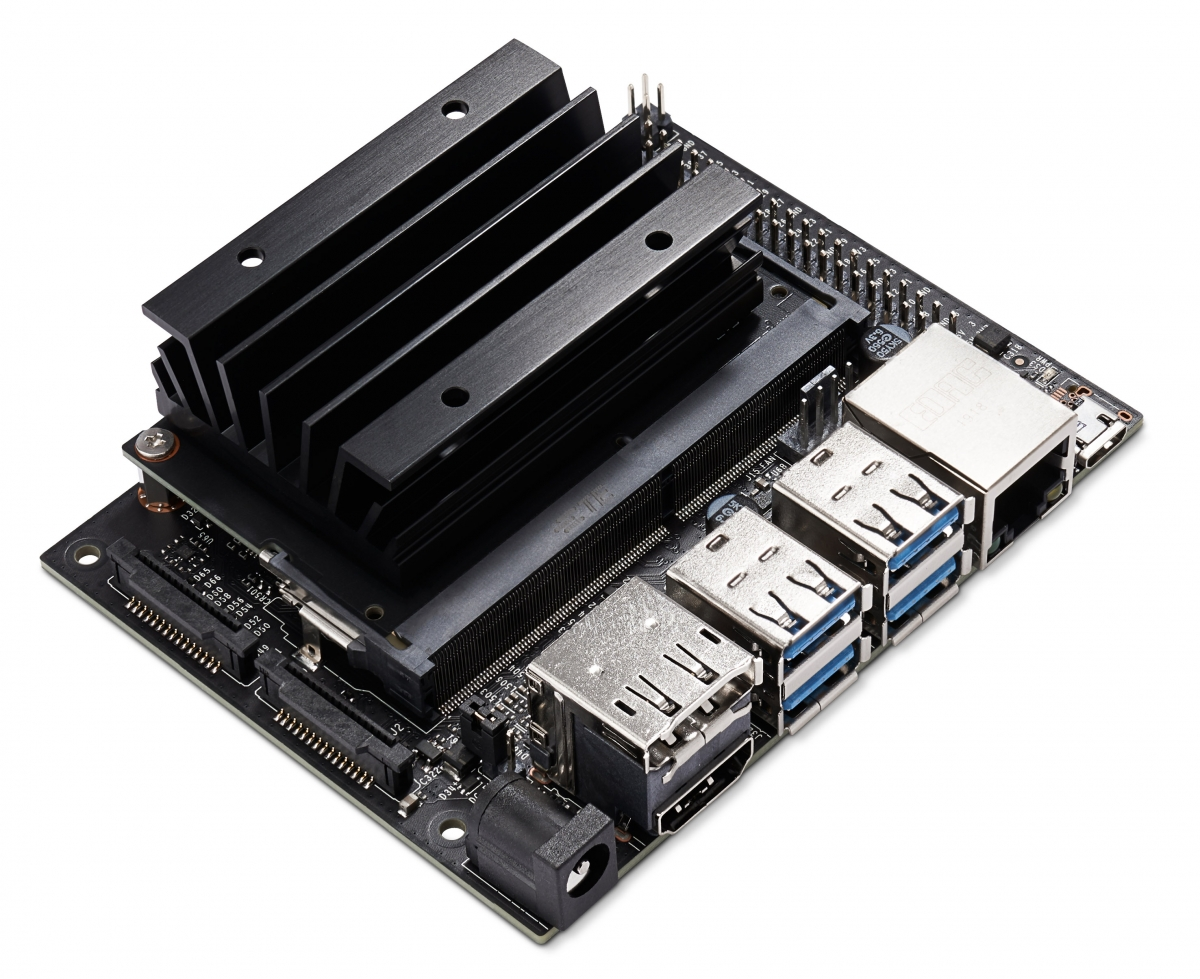
\includegraphics[width=0.9\linewidth]{Bilder/jetson-nano.jpg}
    \end{subfigure}
    \begin{subfigure}{0.5\textwidth}
        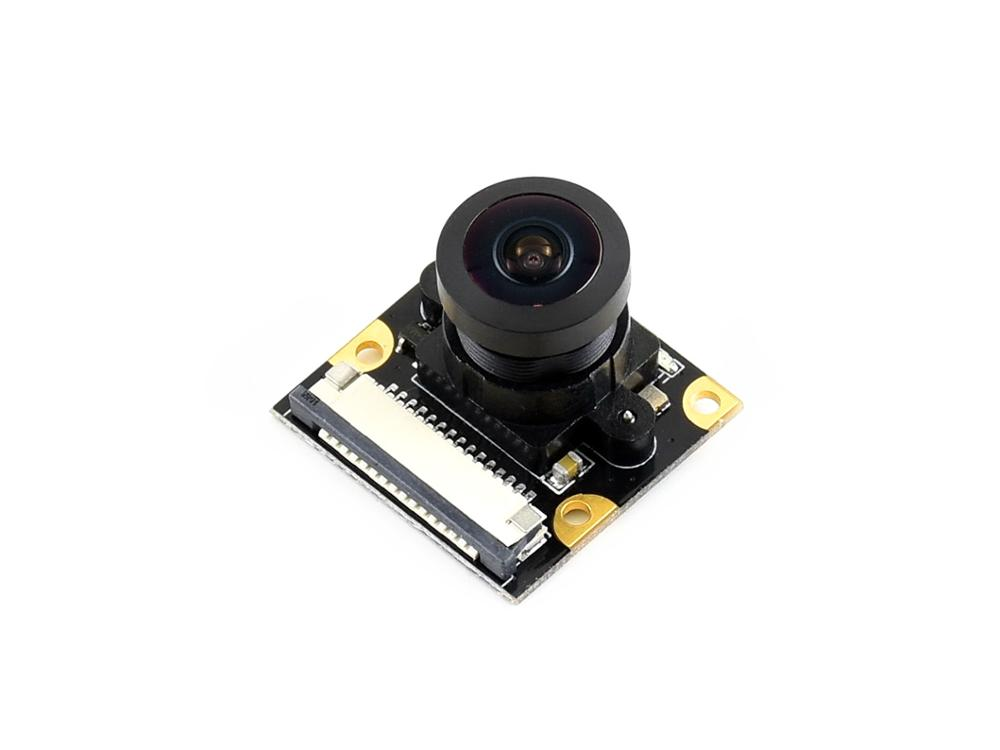
\includegraphics[width=0.9\linewidth]{Bilder/kamera.jpg}
    \end{subfigure}
    \label{fig:Bild3.1}
    \caption[Jetson Nano und Weitwinkelkamera]{Jetson Nano Mikrocontroller und $160^\circ$ Weitwinkelkamera}
\end{figure}

\begin{table}[H]
    \footnotesize
    \begin{longtable}[c]{|l|l|l|l|}
    	\hline
    	\textbf{Nr.} & \textbf{Bauteil}   & \textbf{Anzahl} & \textbf{Bemerkung}                \\ \hline
    	\endfirsthead
    	%
    	\endhead
    	%
    	1            & Jetson Nano        & 1               & 4\,GB RAM Variante                \\
    	2            & Mikro SD Karte     & 1               & mind. 64\,GB                      \\
    	3            & Karosserie         & 1               & ---                               \\
    	4            & Kamera-Befestigung & 1               & ---                               \\
    	5            & Abstandshalter für Kamera aus Acryl & 1 & ---                            \\
        6            & Kamera             & 1               & IMX219-160 Weitwinkel             \\
        7            & WLAN-Stick         & 1               & RTL8121 Chipsatz                  \\
        8            & Erweiterungsboard  & 1               & für Jetson Nano                   \\
        9            & Motor              & 2               & \glqq TT\grqq-Bauform             \\
        10           & Rad                & 2               & 60mm Durchmesser                  \\
        11           & Kugelrolle         & 2               & 1'' Durchmesser                   \\
        12           & Steckeradapter EU  & 1               & ---                               \\
    	13           & Ladegerät          & 1               & 12.6 V                            \\
    	14           & Gamepad            & 1               & kabellos                          \\
    	15           & Montagewerkzeug    & 2               & Schraubenzieher                   \\
    	16           & 6-Pin Kabel        & 1               & 9 cm                              \\
    	17           & Schrauben          & 38              & M2 und M3 Gewinde                 \\
    	18           & Lüfter             & 1               & Bauform 4010                      \\
    	19           & SD-Kartenlesegerät & 1               & ---                               \\ \hline
    	\caption[Materialliste]{Auflistung der benötigten Bauteile für den Aufbau des Jetbot}
    	\label{tab:Tabelle3.1}
    \end{longtable}
\end{table}

\begin{figure}[H]
    \centering
    \fbox{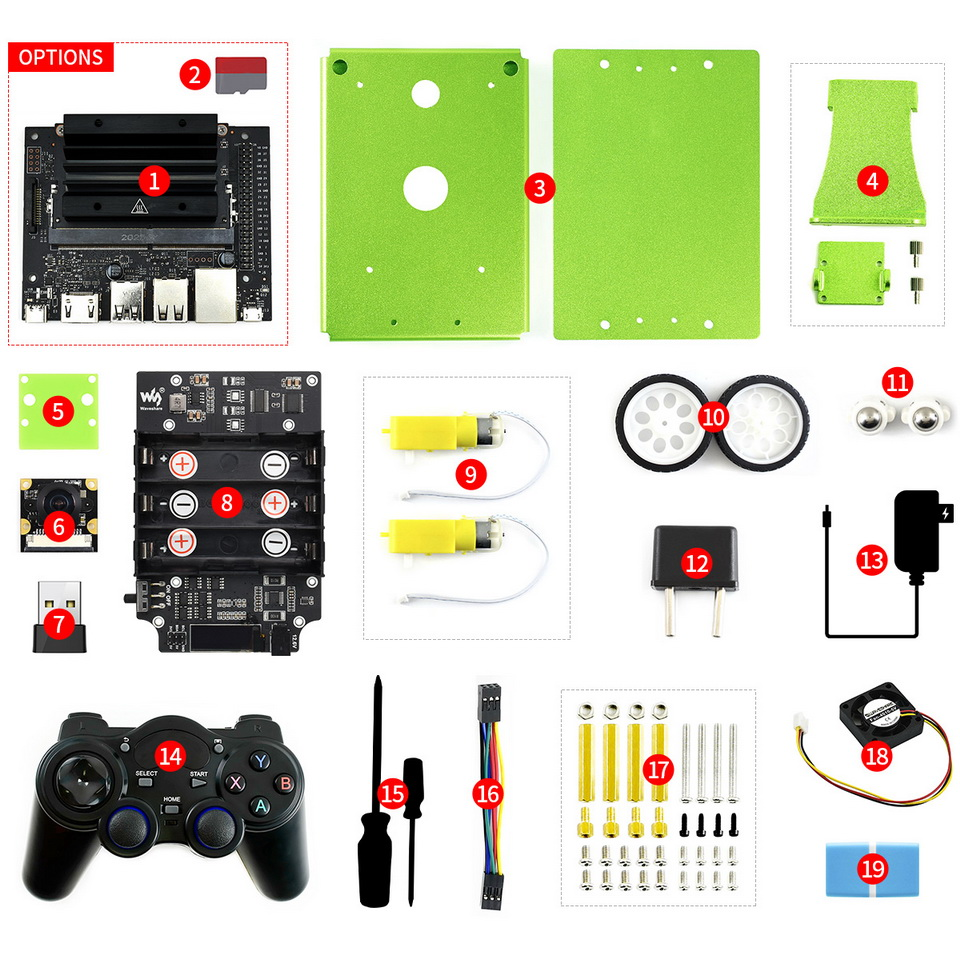
\includegraphics[width=0.53\textwidth]{Bilder/komponenten.jpg}}
    \caption[Komponenten Jetbot]{Darstellung aller verwendeten Komponenten für die Montage des Jetbots}
    \label{fig:Bild3.2}
\end{figure}

\subsection{Hardware-Setup}

Zunächst werden die Motoren auf der Grundfläche des Gehäuses verschraubt. Dieses kann nachfolgen geschlossen werden mit den restlichen Karosserieteilen. Es bietet sich an im nächsten schritt die Räder und Kugelrollen zu montieren, so dass das Gefährt aufrecht stehen kann. Darauf werden die Akkus in dem Erweiterungsboard installiert sowie Abstandshalter an den Ecken angebracht. Das Erweiterungsboard kann dann auf der Karosserie angebracht werden mit vier M2 Schrauben. Auf den im vorherigen Schritt montierten Abstandshaltern wird der Jetson Nano Controller befestigt. Über das 6-Pin Kabel wird anschließend das Erweiterungsboard mit dem Jetson Nano verbunden. Im Anschluss wird der Lüfter auf dem Kühlkörper angebracht und das Lüfterkabel in den PWM-Anschluss gesteckt. Im letzten Schritt wird die Kamerabefestigung am Gehäuse angebracht, der Abstandshalter aus Acryl an an dieser angeschraubt und Abschließend die Kamera montiert. \autoref{fig:Bild3.3} zeigt den fertigen Aufbau des Jetbot Roboterfahrzeugs.

\begin{figure}[H]
    \centering
    \fbox{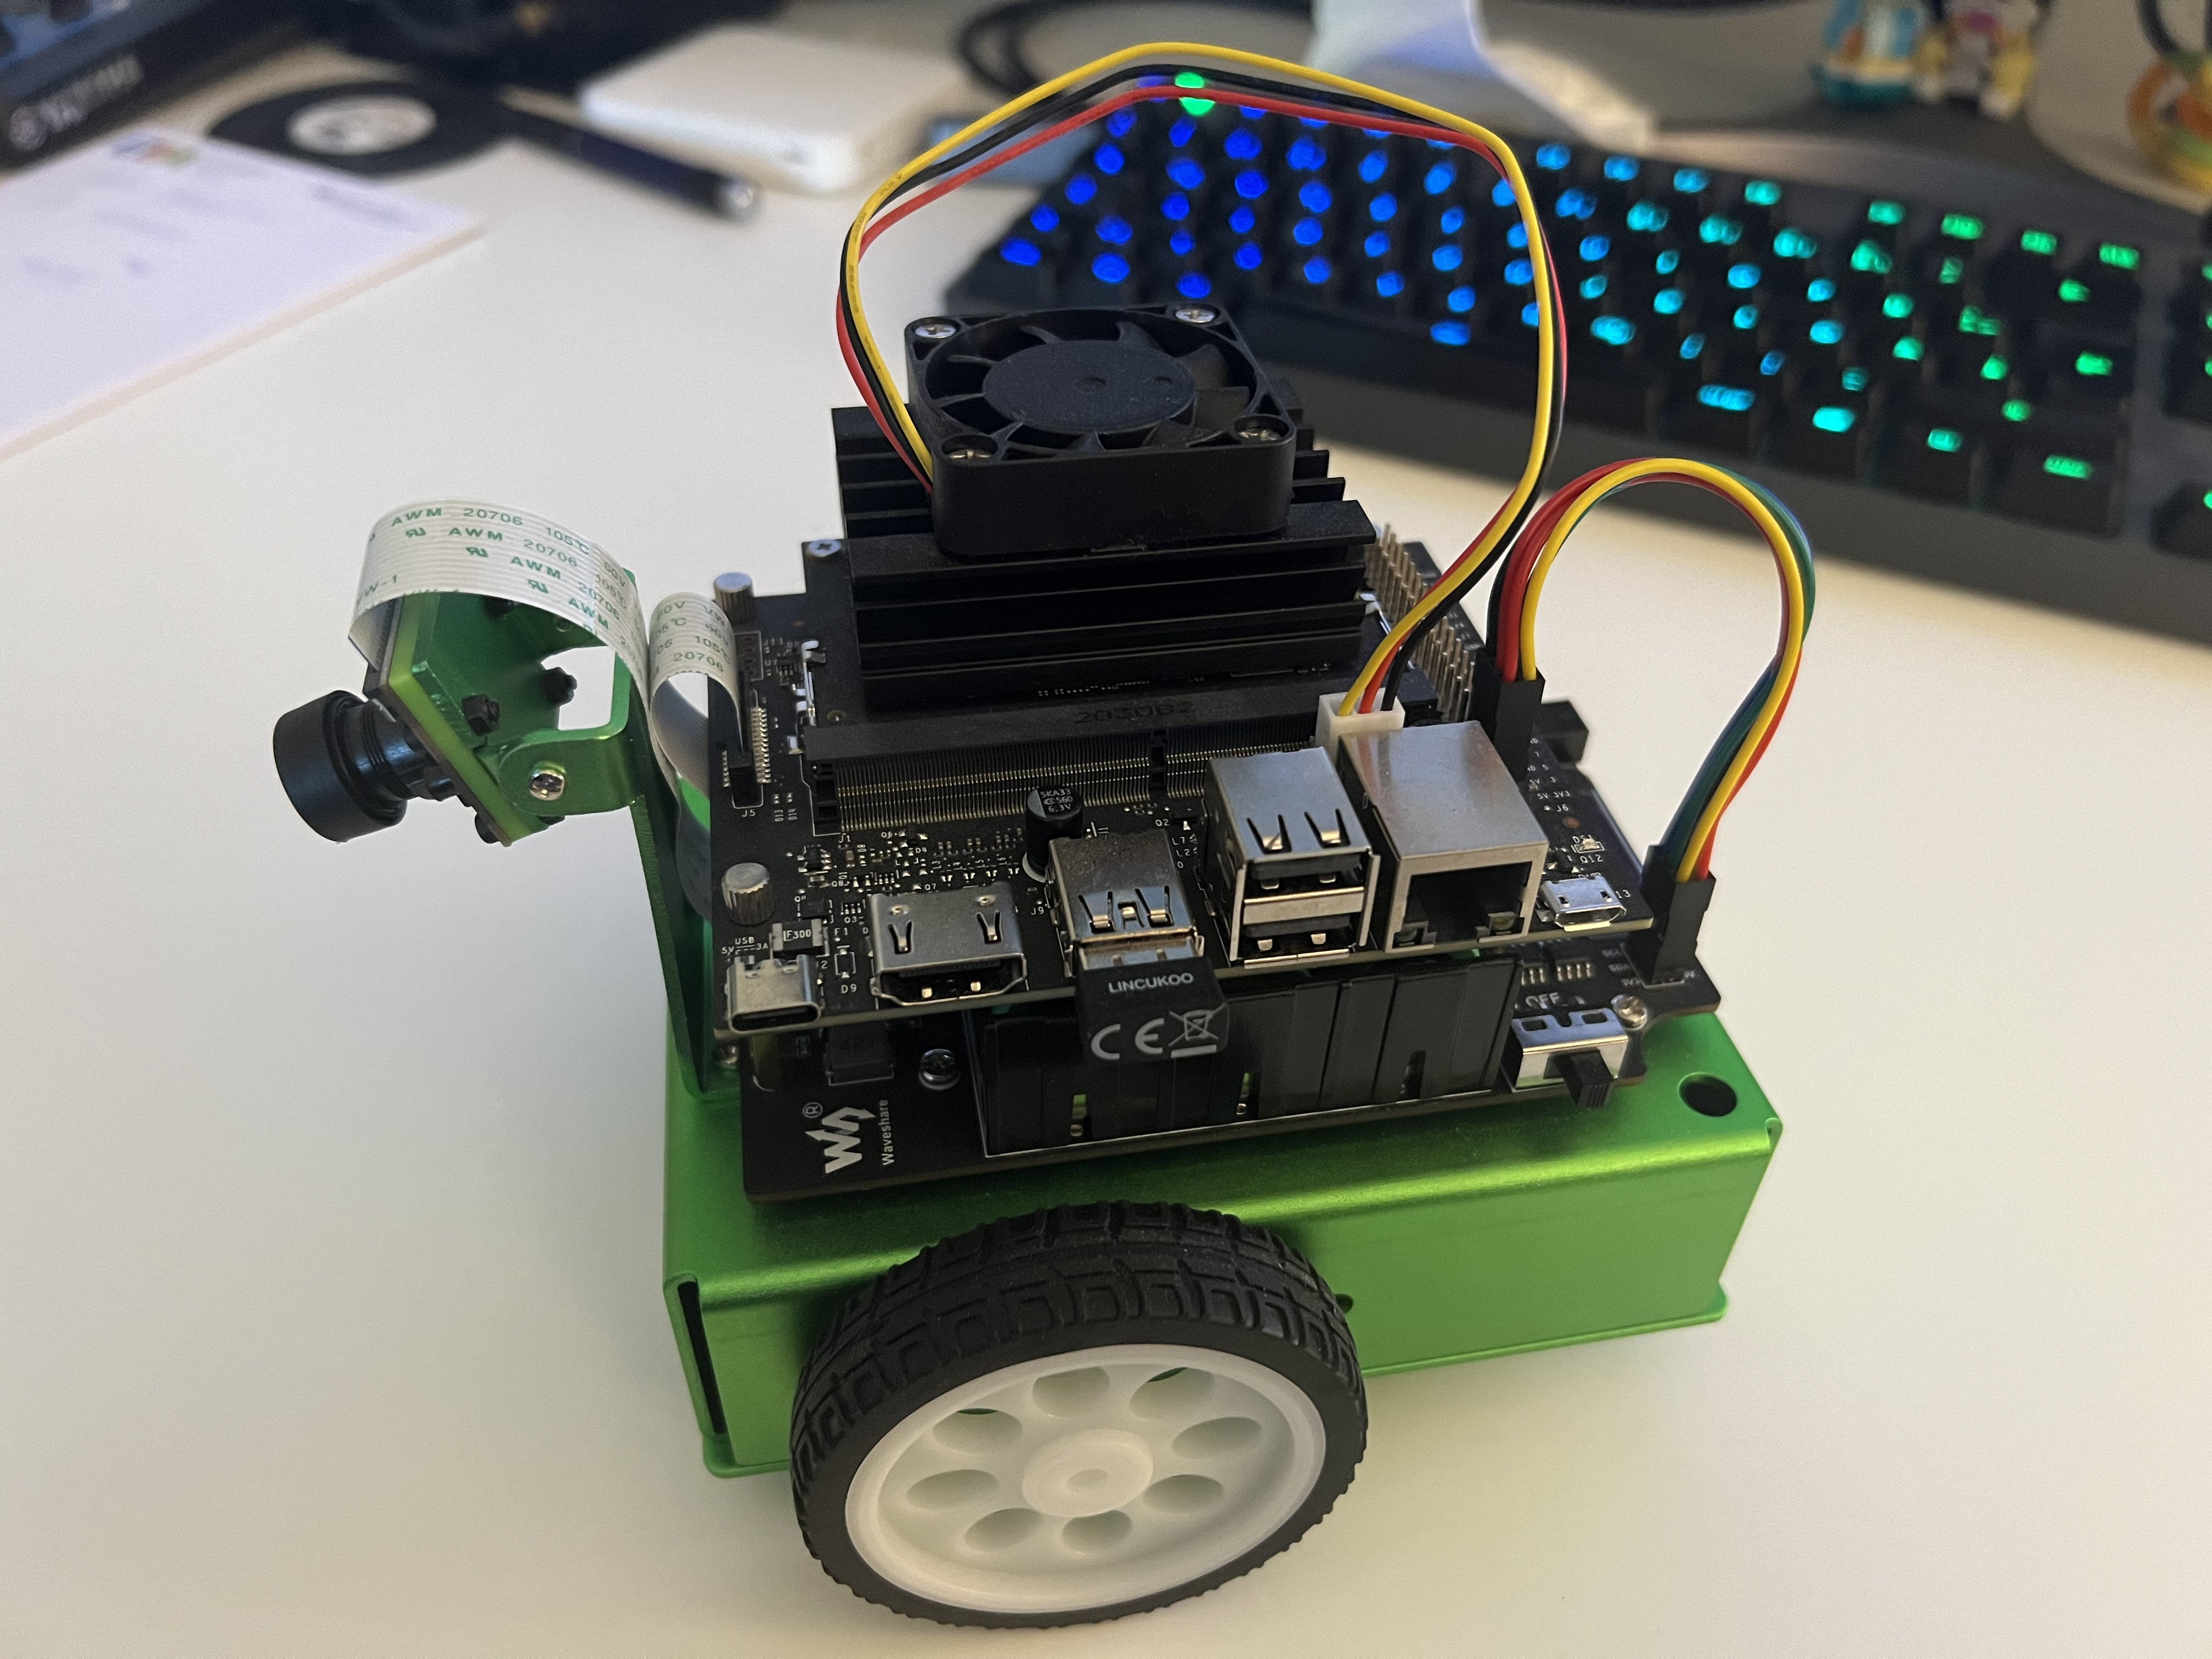
\includegraphics[width=0.98\textwidth]{Bilder/jetbot-aufbau.jpg}}
    \caption[Aufbau Jetbot]{Aufbau des Jetbot-Roboterfahrzeugs}
    \label{fig:Bild3.3}
\end{figure}

\subsection{Software-Setup}

Der erste Schritt ist es sich ein von Nvidia für den Jetson Nano bereitgestelltes Image auf die SD-Karte herunterzuladen. Dieses beinhaltet Ubuntu Linux als Betriebssystem, sämtliche notwendigen Treiber für die Betriebsmittel wie \zB die Kamera und besitzt bereits eine Installation für Python inklusive Jupyter und PyTorch. Worum es sich dabei handelt wird in \autoref{sec:durchführung} geklärt.\\
Die folgenden Schritte sind notwendig, um das Image auf die SD-Karte zu spielen:

\begin{enumerate}
    \item SD-Karte über Lesegerät an beliebigen PC anschließen.
    \item Mit Etcher das heruntergeladene Image auswählen und auf die SD-Karte übertragen.
    \item SD-Karte in den Jetson Nano einstecken.
\end{enumerate}

Der nächste Schritt kann abweichen je nach gewählter Methode. Grundsätzlich ist das Ziel den Jetson Nano mit einem WLAN-Netzwerk zu verbinden. Dazu kann entweder ein Monitor an den HDMI-Port, sowie Maus und Tastatur per USB angeschlossen werden. Nach dem Booten des Systems ist es dann möglich über die Netzwerkeinstellungen eine Verbindung zum WLAN herzustellen. Alternativ ist es möglich über \zB Putty unter Windows oder über das Terminal in Linux oder MACOS auf den Jetson Nano zuzugreifen. Anschließend wird die Verbindung hergestellt über das Kommando\\

\texttt{sudo nmcli device wifi connect <SSID> password <PASSWORD>}. \\

Der Mikrocontroller verbindet sich nun nach dem Einschalten automatisch mit dem ausgewählten Netzwerk. Nachfolgend kann der Jetbot über den Browser eines beliebigen Endgerätes genutzt werden. Dazu sind folgende Schritte notwendig:

\begin{enumerate}
    \item Jetbot einschalten über den Power-Schalter
    \item Warten, bis der Bootvorgang abgeschlossen ist
    \item Die IP-Adresse am piOLED-Display ablesen
    \item Über den Browser eines beliebigen Gerätes im selben Netzwerk navigieren zu \\\texttt{http://<jetbot_ip_address>:8888}
    \item Einloggen mit dem Passwort \texttt{jetbot}
\end{enumerate}

Nachdem über den Browser erfolgreich eine Verbindung hergestellt wurde, wird die Ansicht aus \autoref{fig:Bild3.4} gezeigt.

\begin{figure}[H]
    \centering
    \fbox{\includegraphics[width=0.98\textwidth]{Bilder/oberfläche.png}}
    \caption[Jetbot Bedienoberfläche]{Bedienoberfläche des Jetbots über JupyterLab}
    \label{fig:Bild3.4}
\end{figure}

Zu sehen ist die Oberfläche JupyterLab. Dabei handelt es sich um ein Interface für Jupyter Notebooks. Solch ein Notebook ist grundsätzlich ein aus dem Web aufrufbares Python-Programm. Python meint hier die Programmiersprache in der Version 3.X. Das besondere an einem Jupyter Notebook ist, dass der Code in diesem nicht zwangsläufig in der gegebenen Reihenfolge ausgeführt werden muss. Weiterhin werden bereits berechnete Ergebnisse gespeichert und können zu jedem Zeitpunkt weiter genutzt werden, ohne das ein erneutes Ausführen nötig ist. Das ist besonders hilfreich bei dem Trainieren von neuronalen Netzen, da ein Code-Segment mitunter Stunden oder Tage braucht, um abgearbeitet zu werden. Müsste dies jedes Mal auf ein neues geschehen, würde das viel Zeit in Anspruch nehmen. \autoref{fig:Bild3.5} zeigt ein beispielhaftes Notebook. Als weiterer Vorteil ist zu erkennen, dass ebenso Text wie Code eingebunden werden kann. Somit bietet es sich an die Dokumentation \bzw Beschreibung des Programms in der selben Datei vorzunehmen. Mit Ausblick auf die Programme in den umgesetzten Notebooks für den Jetbot ist zu erwähnen, dass dies dort ebenso vorgenommen wurde. Sämtliche Jupyter Notebooks für die Umsetzung der Kollisionsvermeidung sind im Anhang zu finden.

\begin{figure}[H]
    \centering
    \fbox{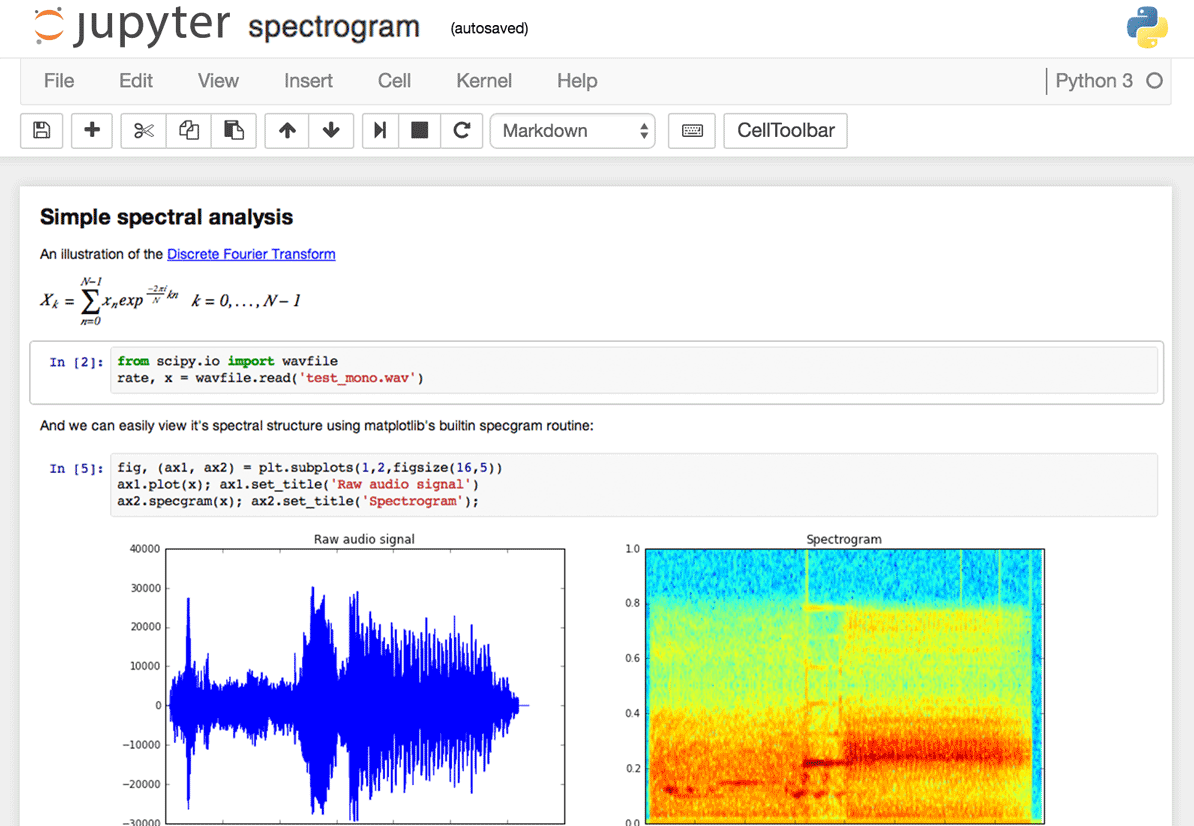
\includegraphics[width=0.98\textwidth]{Bilder/jupyter.png}}
    \caption[Jupyter Notebook]{Beispielhafte Abbildung eines Jupyter Notebooks mit Python-Code und Beschreibung in Textform}
    \label{fig:Bild3.5}
\end{figure}

\include{4_durchführung}

\section{Ergebnisse und Fazit} \label{sec:ergebnisse}

Das gesetzte Ziel, ein kleines Roboterfahrzeug zu befähigen über CNN's frei im Raum zu fahren, ohne dabei mit Hindernissen zu kollidieren, konnte erreicht werden. Dabei wurden als Grundlage die Fragen beantwortet, was ein Convolutional neural Network (CNN) ist, wie diese aufgebaut sind und warum Transfer Learning eine gute Wahl ist, um schnell mit wenig Trainingsdaten ein Modell bezüglich bestimmter Fähigkeiten anzulernen.\\
Jedoch muss festgehalten werden, dass es nur in den meisten Fällen möglich war Kollisionen zu vermeiden. Besonders schlecht beleuchtete Umgebungen oder unbekannte Gebiete in der Wohnung sorgten für erhöhte Fehlerraten, wo Kollisionen nicht vermieden werden konnten. Das Konzept scheint also in diesem simplen Ansatz nicht auf ein realen Verkehrsteilnehmer übertragbar zu sein. Dafür müsste das Modell deutlich intensiver mit mehr Bildern aber auch mehr Klassen trainiert werden, um Situationen \bzw Szenarien besser differenzieren und einschätzen zu können.\\
Dennoch konnte nachgewiesen werden, dass es mit wenigen Zeilen Code bereits möglich ist eine fähige künstliche Intelligenz zu implementieren, die einfache Aufgaben zuverlässig umsetzen kann.

\begin{wrapfigure}{r}{0.64\textwidth}
    \centering
    \fbox{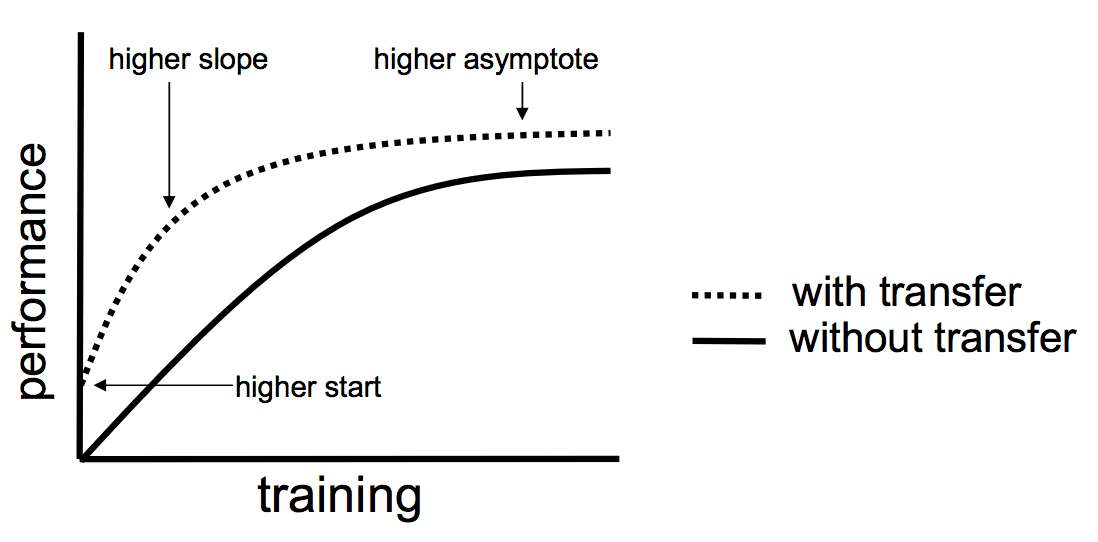
\includegraphics[width=0.62\textwidth]{Bilder/transfer-learning.png}}
    \caption[Vorteile des Transfer Learning]{Vorteile des Transfer Learning \cite{Brownlee2017}}
    \label{fig:Bild5.1}
\end{wrapfigure}

Weiterhin hat sich gezeigt, dass die Nutzung von CNN's mit mehr Layern (\zB ResNet50) dafür sorgt, dass die antrainierten Modelle akkurater werden. Jedoch erhöhen sich damit auch die Anforderungen an die Hardware, insbesondere die GPU. Es konnte festgestellt werden, dass die Reaktionszeit des Jetbots sichtbar langsamer war, desto komplexer das genutzte neuronale Netz ist. Das AlexNet hat sich als Sweetspot erwiesen mit dem gewählten Jetson Nano. Es gibts jedoch bereits heute schon sehr kompakte und deutlich effizientere Mikrocontroller (meist von Nvidia) die eine tausendfache Leistung im Vergleich zu der genutzten Hardware haben. \\
Das Pre-Training hat sich hingegen als eine kleinere Herausforderung dargestellt, da dieses auf einem separaten Computer stattfinden konnte, welcher mit einer Hochleistungsgrafikkarte (Nvidia RTX 3090) ausgestattet ist.

\section{Ausblick} \label{sec:ausblick}

\section{Anhang} \label{sec:anhang}

%---------Quellen---------------------------------
\newpage
\section*{Literaturverzeichnis}
\addcontentsline{toc}{section}{Literaturverzeichnis}

\nocite{Styczynski2017}
\nocite{Prakash2021}
\nocite{Amaratunga2020}
\nocite{Kalaiarasi2020}

\printbibliography[
	heading=subbibintoc,
	type=book,
	title={Bücher}
]

\nocite{Schaeffer2021}
\nocite{Borchers2022}

\printbibliography[
	heading=subbibintoc,
	type=article,
	title={Artikel}
]

\nocite{Wikimedia2014}
\nocite{Regensburg2018}
\nocite{Woelki2020}
\nocite{Wuttke}
\nocite{Wuertz2019}
\nocite{Wikipedia2022}
\nocite{Vasudevan2020}
\nocite{Sonwane2020}

\printbibliography[
	heading=subbibintoc,
	type=online,
	title={Online Quellen}
]

\end{document}
